

\clearpage
\section{Einleitung}
\vspace*{\fill}
\begin{center}
\begin{minipage}{.6\textwidth}

Vorliegende Arbeit entstand im Rahmen meiner Werkstudententätigkeit bei der Firma i-Ways Sales Solutions GmbH und meinem Mitwirken
an der von i-Ways entwickelten, auf einem PHP-Webframework basierenden Multichannel-Marketing Software iTool3, die es -- unter Anderem -- gestattet über eine Weboberfläche Produkte verschiedener
Verkäufer auf Onlinemarktplätzen wie Amazon oder eBay anzubieten.
Ziel dieser Arbeit ist es die Anwendung, im Kundenauftrag, um die Möglichkeit der Anbindung an den Mercateo Marktplatz, einer Online B2B Beschaffungsplattform, zu erweitern.
Da Mercateo ein API bereitstellt das Produktdaten über einen XML-Katalog empfängt, soll im folgenden untersucht werden, wie die Anbindung der Software iTool3 an den Mercateo Marktplatz realisiert werden kann. Ziel der Arbeit ist es einen funktionsfähigen Prototypen zu entwickeln, der einen fehlerfreien Transfer der mit iTool verwalteten Produkte an Mercateo ermöglicht.
\end{minipage}
\end{center}
\vfill % equivalent to \vspace{\fill}
\clearpage

\pagebreak

\section{Grundlagen}

%erst Cake, dann itool
	
	\subsection{iTool3}
	
	iTool3 ist eine auf dem CakePHP 3.3 - Framework basierende eCommerce Software Lösung zur Steuerung von Produktsortimenten auf verschiedenen Marktplätzen mit dem Ziel, den
	Vertriebsprozess zu automatisieren. Es ermöglicht dem Nutzer, über eine einzelne Benutzeroberfläche, Produkte auf Marktplätzen wie eBay, Amazon oder auch einem Magento-Store
	zu verwalten. Produkte können dabei händisch erstellt oder aus bestehenden Datenquellen in die Software	eingepflegt werden. Im Anschluss ist es möglich diese Produkte auf einem oder mehreren Marktplätzen anzubieten. Die Verwaltung und Abwicklung der eingehenden Bestellungen läuft dabei komplett über das iTool.
	Da für jeden Marktplatz unterschiedliche Daten benötigt werden um auf ihm erfolgreich zu verkaufen, können für jedes Produkt unterschiedliche Attribute mit wiederum unterschiedlichen Werten angelegt werden. Die Produktverwaltung der Software folgt daher dem Entity-Attribute-Value Modell.
	
	
	\subsubsection{Verkäufer und Benutzer}
	
	Es wird unterschieden zwischen Verkäufern (Core-Seller) und Benutzern (Core-User). Einem Verkäufer können mehrere Benutzer zugeordnet werden, die, mit mehr oder weniger Rechten ausgestattet, die Produkte nur einsehen, oder Kontrolle über die gesamte Produkt- und Bestellverwaltung haben können.\\
	\begin{minipage}{\linewidth}
		\vspace{1em}
		\centering
		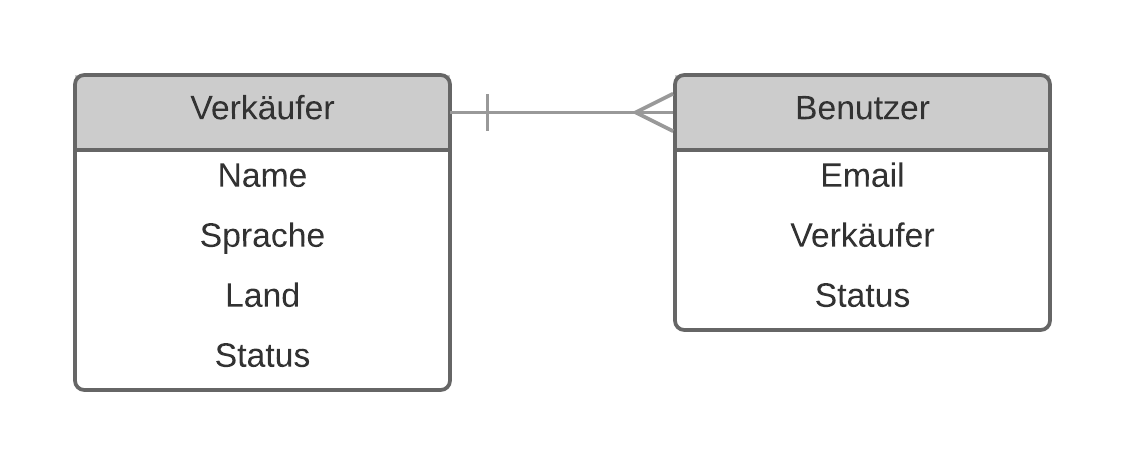
\includegraphics[width=0.6\linewidth]{img/ERD_Seller_User_complete}
		\captionof{figure}[ERD]{ER-Diagramm: Verkäufer - Benutzer}
		\label{fig:header}
		\vspace{1em}
	\end{minipage}
	
	Benutzerdaten werden dabei in der Tabelle \texttt{core\_users} gespeichert, Verkäuferdaten in \texttt{core\_sellers}.

	 
	
	\subsubsection{Produktverwaltung}
	
	Die Produktverwaltung ist aufgeteilt in Produkte und Kategorien. \textbf{Produkte} besitzen Attribute wie Titel, Preis, Beschreibung etc. die für jeden Marktplatz auf denen diese angeboten werden sollen unterschiedlich ausfallen können. Es kann gewählt werden, ob ein Produkt auf einem bestimmten Marktplatz angeboten werden soll oder nicht. Ein Produkt kann dabei mehreren \textbf{Kategorien} zugeordnet sein.\\
	\begin{minipage}{\linewidth}
		\vspace{1em}
		\centering
		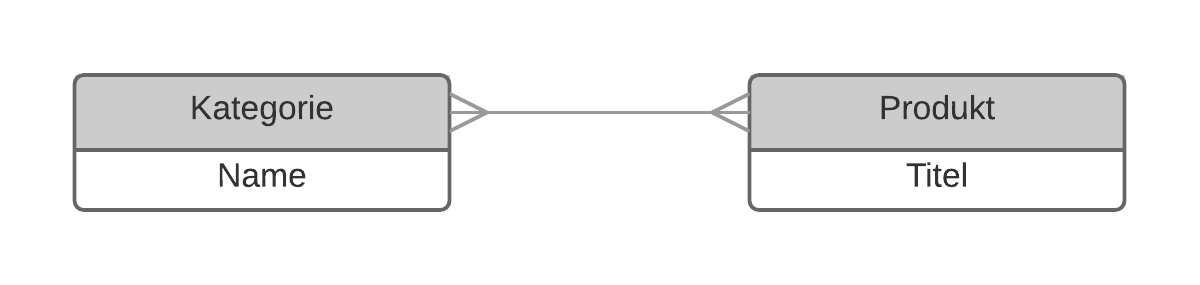
\includegraphics[width=0.6\linewidth]{img/ERD_Category_Product}
		\captionof{figure}[ERD]{ER-Diagramm: Kategorie - Produkt}
		\label{fig:header}
		\vspace{1em}
	\end{minipage}
	Eine Kind-Kategorie hat jeweils genau eine Eltern-Kategorie. Eine Eltern-Kategorie kann jedoch mehrere Kind\_Kategorien haben.Die  einzelnen Produkte sind genau einem Verkäufer zugeordnet. \\
	\begin{minipage}{\linewidth}
		\vspace{1em}
		\centering
		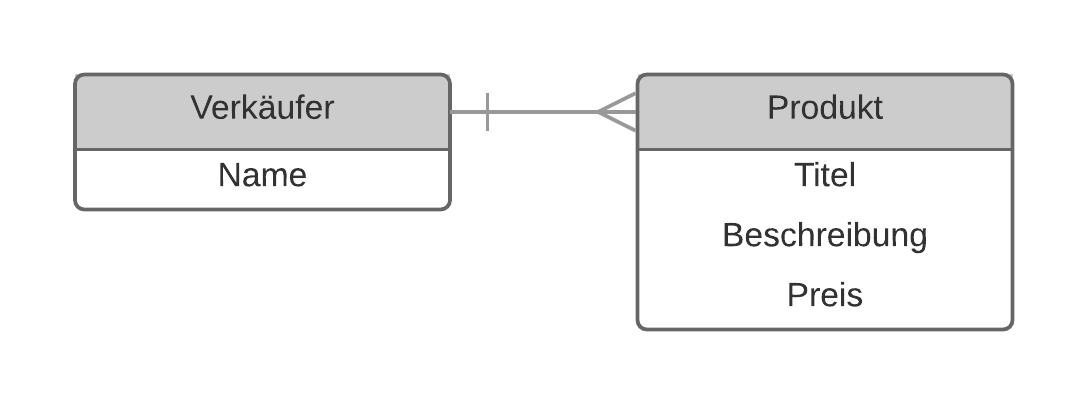
\includegraphics[width=0.6\linewidth]{img/ERD_Seller_Product}
		\captionof{figure}[ERD]{ER-Diagramm: Verkäufer - Benutzer}
		\label{fig:header}
		\vspace{1em}
	\end{minipage}
	
	Alle Produktdaten sind in der Tabelle \texttt{core\_products} und den damit verknüpften Tabellen hinterlegt.
	
	\subsubsection{Dashboard}
	
	Auf dem Dashboard werden Informationen über die Anzahl der insgesamt eingegangenen Bestellungen, den durchschnittlichen Bestellwert, die Gesamtzahl der Kunden, den insgesamt erwirtschafteten Umsatz, eine Übersicht der zuletzt eingegangenen Bestellungen sowie eine graphische Übersicht der während eines Jahres erwirtschafteten Umsätze angezeigt. 
	%Bild einfügen
	
	\subsection{Der BMECat} %Das XML Katalogformat BMECat
	
	Der BMECat ist ein vom \enquote{Bundesverband Materialwirtschaft, Einkauf und Logistik e.V} in Zusammenarbeit mit dem \enquote{eBusiness Standardization Committee} entwickelter XML
	Standard mit dem Ziel den Austausch von Produktkatalogen zwischen Lieferanten und beschaffenden Organisationen zu standardisieren und somit zu vereinfachen\footnote{BMECat V1.2 Spezifikation, Seite 5}. 
	
	\subsubsection{Terminologie}
	Ein \textbf{Produktkatalog} ist die Menge aller benötigten Daten, welche vom katalogerzeugenden Unternehmen an das katalogempfangende Unternehmen übermittelt werden sollen.\\
	Ein \textbf{Katalogdokument} ist eine XML-Datei, in der der Produktkatalog im BMECat-Format gespeichert und zum Katalogemfänger übermittelt wird.\\
	Eine \textbf{Kataloggruppe} ist ein Datenbereich, der eine Gruppe definiert, welcher gleichartige Artikel zugeordnet werden können. Diese wird im BMEcat-Format durch das Element \texttt{\textbf{CATALOG\_STRUCTURE}} abgebildet.\\
	Ein \textbf{Kataloggruppensystem} ist ein hierarchischer Baum von verknüpften Kataloggruppen. Es wird
	im BMEcat-Format durch das Element \texttt{\textbf{CATALOG\_GROUP\_SYSTEM}} abgebildet.\footnote{vgl. hierzu:BMECat V1.2 Spezifikation, Seite 7}
	
	\subsubsection{Transaktionen}
	Im BMECat wird zwischen 3 verschiedenen Transaktionsarten unterschieden:
	\begin{itemize}[noitemsep]
	\item \texttt{\textbf{T\_NEW\_CATALOG}} - Übertragung eines neuen Produktkataloges
	\item \texttt{\textbf{T\_UPDATE\_PRODUCTS}} - Aktualisierung von Produktdaten
	\item \texttt{\textbf{T\_UPDATE\_PRICES}} - Aktualisierung von Preisinformationen
	\end{itemize} 
	Die Unterscheidung geschieht um die Größe eines Katalogdokumentes zu reduzieren. Es muss so z.B. nicht ein kompletter Produktkatalog übertragen werden, falls sich bei einem \(oder mehreren\) Artikel\(n\) der Preis ändert. %crap
	
	\subsubsection{Aufbau}
	
	Ein BMECat-Dokument besteht aus einer Folge von \enquote{Kann} und \enquote{Muss} Feldern, den dazugehörigen Datentypen und Feldlängen und ist folgendermaßen aufgebaut:
		
		\begin{enumerate}
		
			\item 
			XML Deklaration:
			\begin{lstlisting}
			<?xml version="1.0" encoding="UTF-8"?>
			<!DOCTYPE BMECAT SYSTEM "bmecat_new_catalog.dtd">
			<BMECAT version="1.2" xml:lang="de" xmlns="http://www.bmecat.org/bmecat/1.2/bmecat_new_catalog">
			\end{lstlisting}
			
			\item
			Header-Bereich (mit Informationen über Kataloganbieter und Empfänger, Bezeichnung und Erstellungsdatum des Kataloges etc.  )
			\begin{lstlisting} %vernünftige Daten
			<HEADER> 
			  <GENERATOR_INFO> Kann </GENERATOR_INFO>
			  <CATALOG> Muss </CATALOG>
			  <BUYER> Kann </BUYER>
			  <SUPPLIER> Muss </SUPPLIER>
			</HEADER>
			\end{lstlisting}
			\pagebreak
			\item Produktgruppensystem (Baumstruktur der Produktgruppen mit den Attributwerten \enquote{root}, \texttt{Node} und \textit{Leaf})
			\begin{lstlisting}
			<CATALOG_STRUCTURE type="root">
			   <GROUP_ID>1</GROUP_ID>
			   <GROUP_NAME>Katalog</GROUP_NAME>
			   <PARENT_ID>0</PARENT_ID>
			   <GROUP_ORDER>1</GROUP_ORDER>
			</CATALOG_STRUCTURE>
			  <CATALOG_STRUCTURE type="node">
			   <GROUP_ID>2</GROUP_ID>
			   <GROUP_NAME>Spiele &amp; Konsolen</GROUP_NAME>
			   <PARENT_ID>1</PARENT_ID>
			 </CATALOG_STRUCTURE>
			 <CATALOG_STRUCTURE type="leaf">
			   <GROUP_ID>7</GROUP_ID>
			   <GROUP_NAME>PlayStation 4</GROUP_NAME>
			   <PARENT_ID>2</PARENT_ID>
			 </CATALOG_STRUCTURE>
			\end{lstlisting}
			
			
			
			\item Artikel (mit Attributen und Werten)
			
			\begin{lstlisting}
			<ARTICLE mode="new">
			  <SUPPLIER_AID>9057320097280</SUPPLIER_AID>
			    <ARTICLE_DETAILS>
			      <DESCRIPTION_SHORT>GTA 5</DESCRIPTION_SHORT>
			      <DESCRIPTION_LONG>Das tolle neue Spiel</DESCRIPTION_LONG>
			      <EAN>87126723434</EAN>
				... weitere Attribute ...
			    </ARTICLE_DETAILS>
				...weitere Felder ...
			</ARTICLE>
			\end{lstlisting}
			
	
			\item Zuordnung der Artikel zu den Produktgruppen.
			\begin{lstlisting}
			<ARTICLE_TO_CATALOGGROUP_MAP>
			  <ART_ID>9057320097280</ART_ID>
			  <CATALOG_GROUP_ID>7</CATALOG_GROUP_ID>
			</ARTICLE_TO_CATALOGGROUP_MAP>
			\end{lstlisting}
		
		\end{enumerate}
		
	--- Übersicht der im BMECat verwendeten Datentypen --- noch einfügen ---
	
	Im Folgenden wird jeder Teilbereich mit seinen Unterelementen graphisch dargestellt und erläutert. Farblich rot markiert sind jeweils die \enquote{Muss}-Felder, welche zwingend in einem gültigen BMECat Dokument vorkommen müssen, grün die \enquote{Kann}-Felder. Ein Plus \(+\) Zeichen hinter dem Elementnamen indiziert, dass dieses Element mehrfach an dieser Stelle vorkommen muss, jedoch mindestens einmal. Ein Asterisk \(*\) zeigt an, dass dieses Element einmal, mehrfach oder gar nicht vorkommen kann.  
	
	\textbf{\underline{Header}}\\
	Im Header werden allgemeine Informationen über das Katalogdokument hinterlegt und
	 Default Werte gesetzt. Das Element \texttt{\textbf{CATALOG}} enthält dabei %??
	
	Informationen zur Identifikation und Beschreibung des Produktkataloges, wie z.B. die
	 Katalog\-ID, die Katalogversion oder die für das Katalogdokument geltende Sprache sowie
	  Elemente zum Setzten von Standard-Werten wie z.B. die für das Katalogdokument geltende Währungsangabe \footnote{BMECat V 1.2 Spezifikation, Seite 27,29}.
	
	\begin{minipage}{\linewidth}
		\vspace{1em}
		\centering
		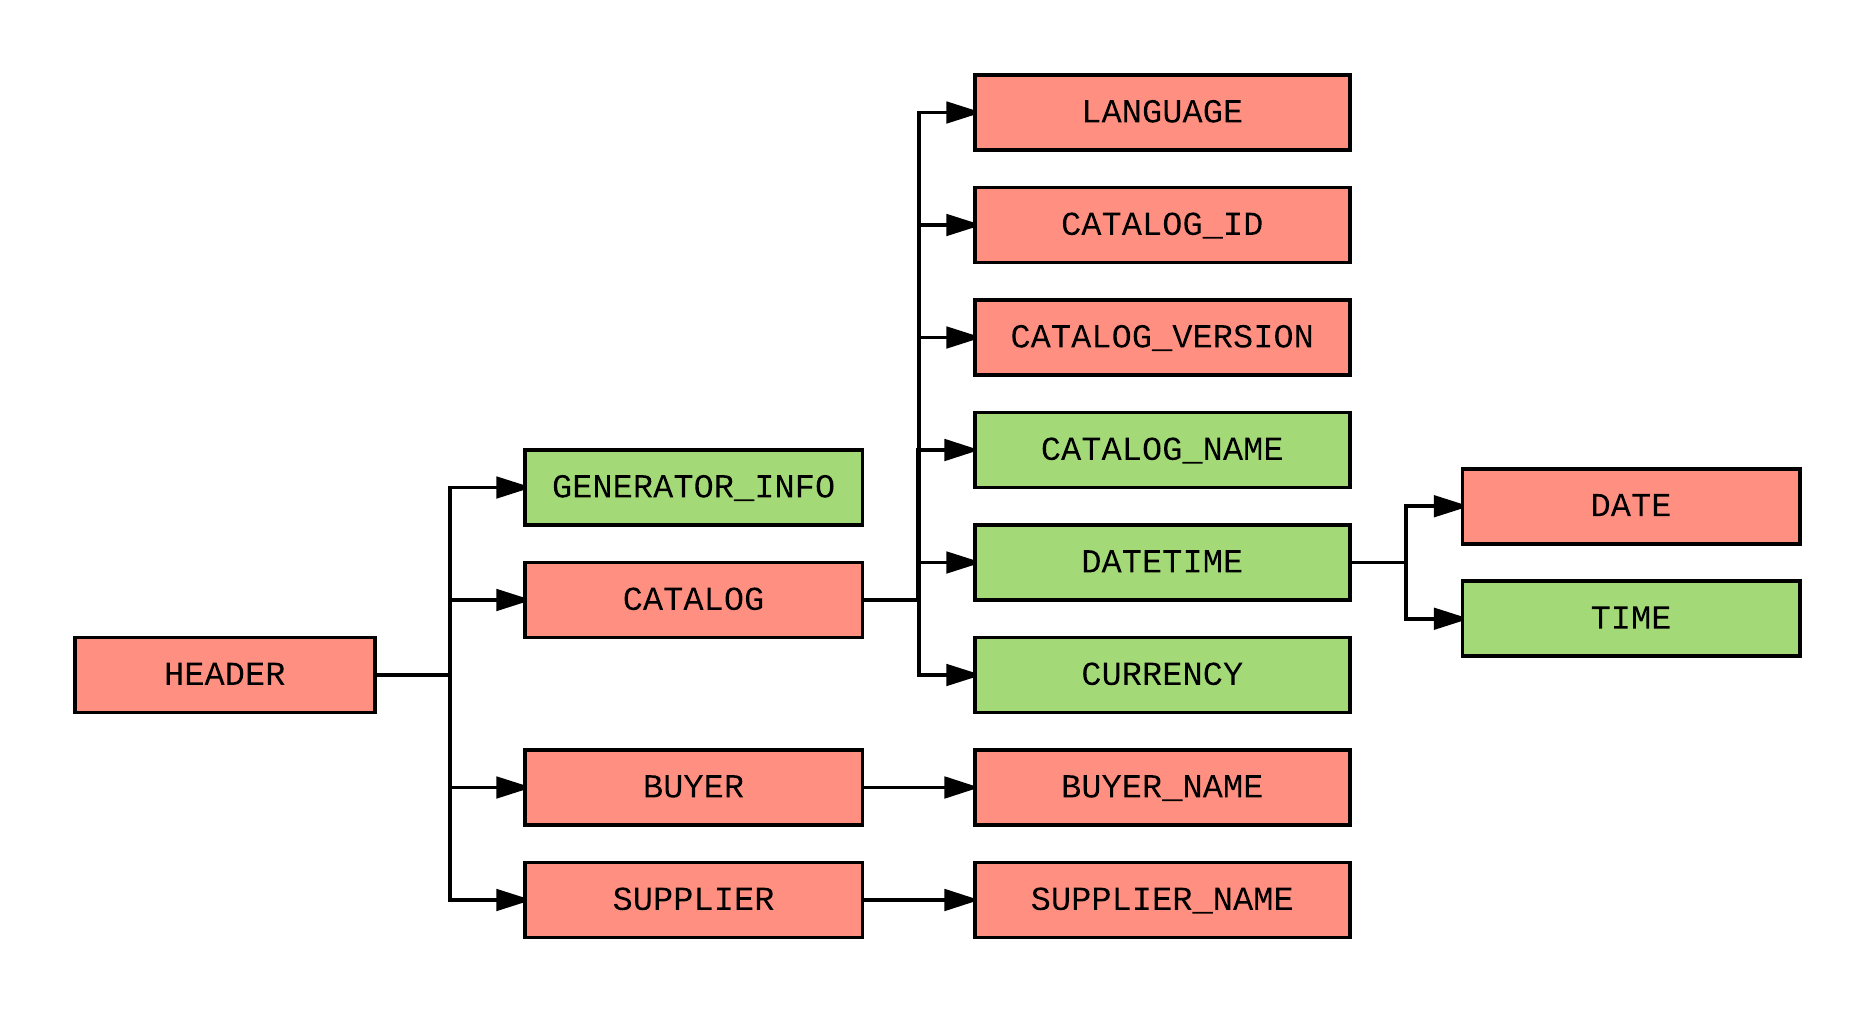
\includegraphics[width=0.85\linewidth]{img/BMECat_Header}
		\captionof{figure}[Headerstruktur]{Headerstruktur}
		\label{fig:header}
		\vspace{1em}
	\end{minipage}
	
	
	
	\textbf{\underline{Die Transaktion T\_NEW\_CATALOG}}
	
	Diese Transaktion wird verwandt, um einen initialen Produktkatalog zu übertragen. Das empfangende System reagiert dabei je nach übertragener \texttt{CATALOG\_ID}, \texttt{CATALOG\_VERSION}
	und \texttt{LANGUAGE} unterschiedlich. Dieser Zusammenhang wir später noch erläutert. %logik
	
	
	\begin{minipage}{\linewidth}
		\vspace{1em}
		\centering
		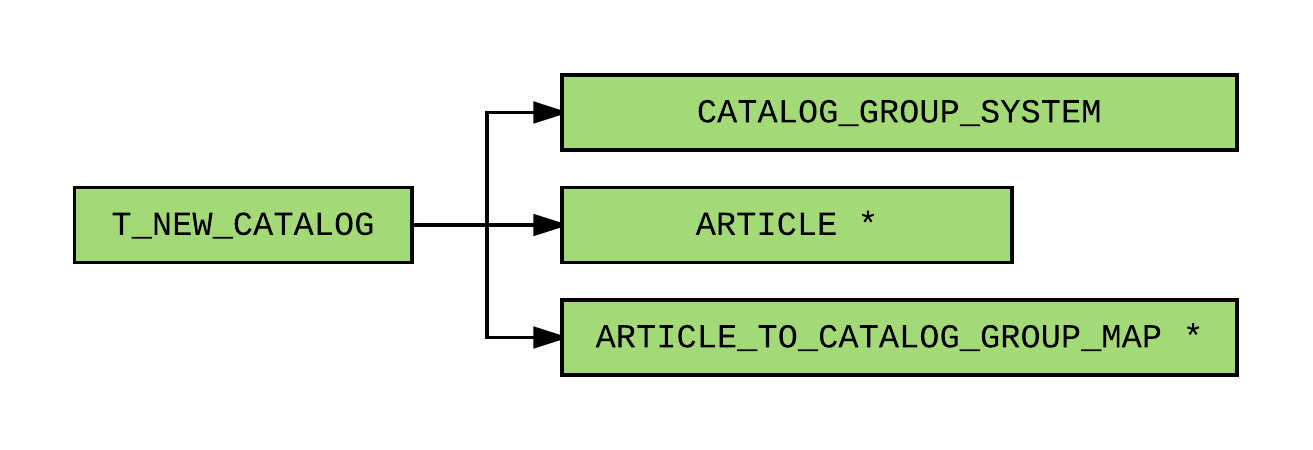
\includegraphics[width=0.65\linewidth]{img/newCatalog}
		\captionof{figure}[T\_NEW\_CATALOG]{T\_NEW\_CATALOG}
		\label{fig:header}
		\vspace{1em}
	\end{minipage}
	
	\textbf{\underline{Die Transaktion T\_UPDATE\_PRODUCTS}}\\
	
	Bei dieser Transaktion werden Artikeldaten übertragen und gegebenenfalls einer Kataloggruppe zugeordnet. Je nach Kennung des Artikels werden die übertragenen
	Artikel im Zielsystem entweder hinzugefügt, gelöscht oder die Artikeldaten werden komplett ersetzt.
	Der Artikel wird immer komplett ausgetauscht, eine Änderung von einzelnen Datenfeldern innerhalb eines Artikels ist nicht möglich.
	Wie der Grafik entnommen werden kann ist bei dieser Transaktion nur die Übertragung von Produktdaten und die Zuordnung von Produkten zu Kataloggruppen möglich, nicht jedoch das Erstellen eines neuen Kataloggruppensytems \footnote{vgl. BMECat V 1.2 Spezifikation, Seite 52}.
	
	\begin{minipage}{\linewidth}
		\vspace{1em}
		\centering
		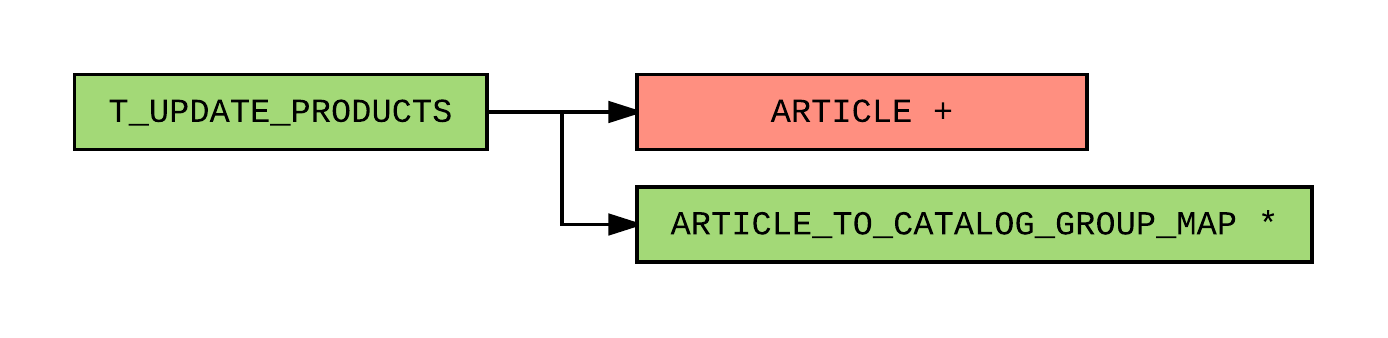
\includegraphics[width=0.65\linewidth]{img/updateProducts}
		\captionof{figure}[T\_UPDATE\_PRODUCTS]{T\_UPDATE\_PRODUCTS}
		\label{fig:header}
		\vspace{1em}
	\end{minipage}
	
	Das Element \texttt{T\_UPDATE\_PRODUCTS} verfügt über das Attribut \texttt{prev\_version}, welches die Anzahl der vorausgegangenen Updates enthält. Der Wert dieses Attributes wird nach jedem Update um 1 erhöht.
	
	\begin{lstlisting}
	<T_UPDATE_PRODUCTS prev_version="91">...</T_UPDATE_PRODUCTS>
	\end{lstlisting}
	
	
	
	\textbf{\underline{Die Elemente CATALOG\_GROUP\_SYSTEM und CATALOG\_STRUCTURE}}\\
	
	Im Element \texttt{CATALOG\_GROUP\_SYSTEM} werden die \texttt{GROUP\_SYSTEM\_ID} und der \texttt{GROUP\_SYSTEM\_NAME} bekannt gemacht sowie die Katalogstruktur -- \texttt{CATALOG\_STRUCTURE} --  beschrieben. Dabei gibt es genau ein Wurzelelement, sowie beliebig viele Knoten und Blätter. Jedes Element hat dabei eine als \texttt{GROUP\_ID} bezeichnete ID und wird über \texttt{PARENT\_ID} die  dem jeweiligen Elternelement zugeordnet. Die Zuordnung der Artikel zu den Artikelgruppen erfolgt mit dem Element \texttt{ARTICLE\_TO\_CATALOG\_GROUP\_MAP} das weiter unten beschrieben wird.
	
	\begin{minipage}{\linewidth}
		\vspace{1em}
		\centering
		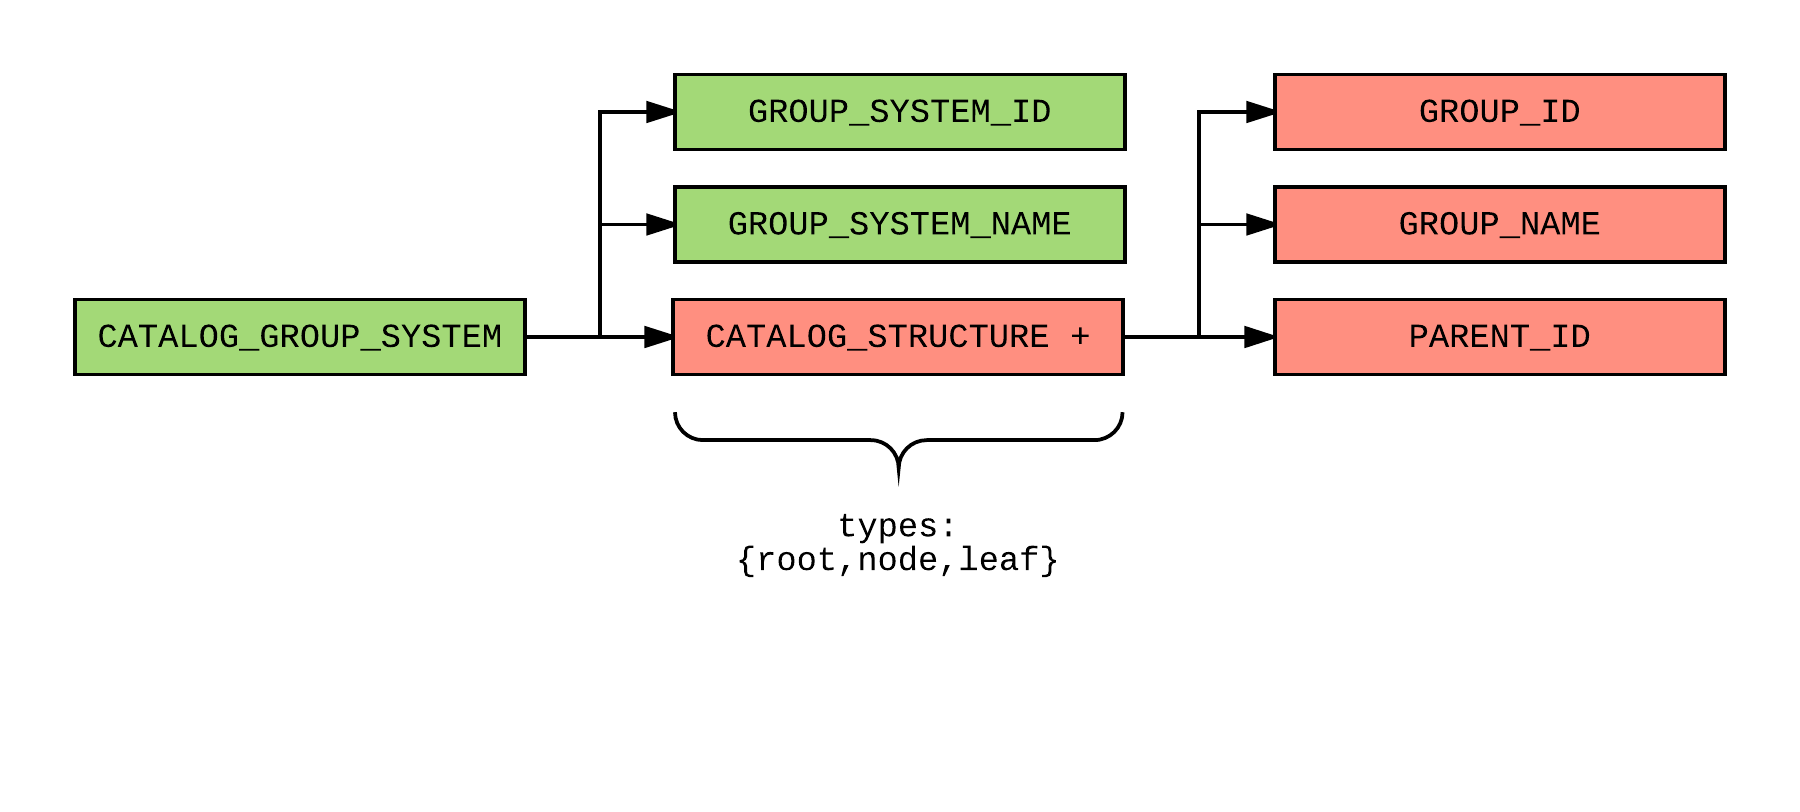
\includegraphics[width=0.85\linewidth]{img/catalogGroupSystem}
		\captionof{figure}[CATALOG\_GROUP\_SYSTEM und CATALOG\_STRUCTURE]{CATALOG\_GROUP\_SYSTEM und CATALOG\_STRUCTURE}
		\label{fig:header}
		\vspace{1em}
	\end{minipage} 
	
	\textbf{\underline{Das Element ARTICLE}}\\
	Das Artikelelement schließlich enthält Informationen über einen Artikel, wie Überschrift, Beschreibung, Bilder, Preisinformationen, eine \textbf{eindeutige} Artikelnummer usw. Die Artikelnummer wird über das Element \texttt{SUPPLIER\_AID} bekanntgegeben, handelt es sich um einen Variantenartikel, so bildet sich die Artikelnummer aus der \texttt{SUPPLIER\_AID} und der \texttt{SUPPLIER\_AID\_SUPPLEMENT}. Dies ist hier jedoch nicht umgesetzt. Die als \textit{eCl@ass} und \textit{Zolltarifnummer} zusammengefassten \texttt{ARTICLE\_FEATURES} werden explizit von Mercateo verlangt.
	
	\begin{minipage}{\linewidth}
		\vspace{1em}
		\centering
		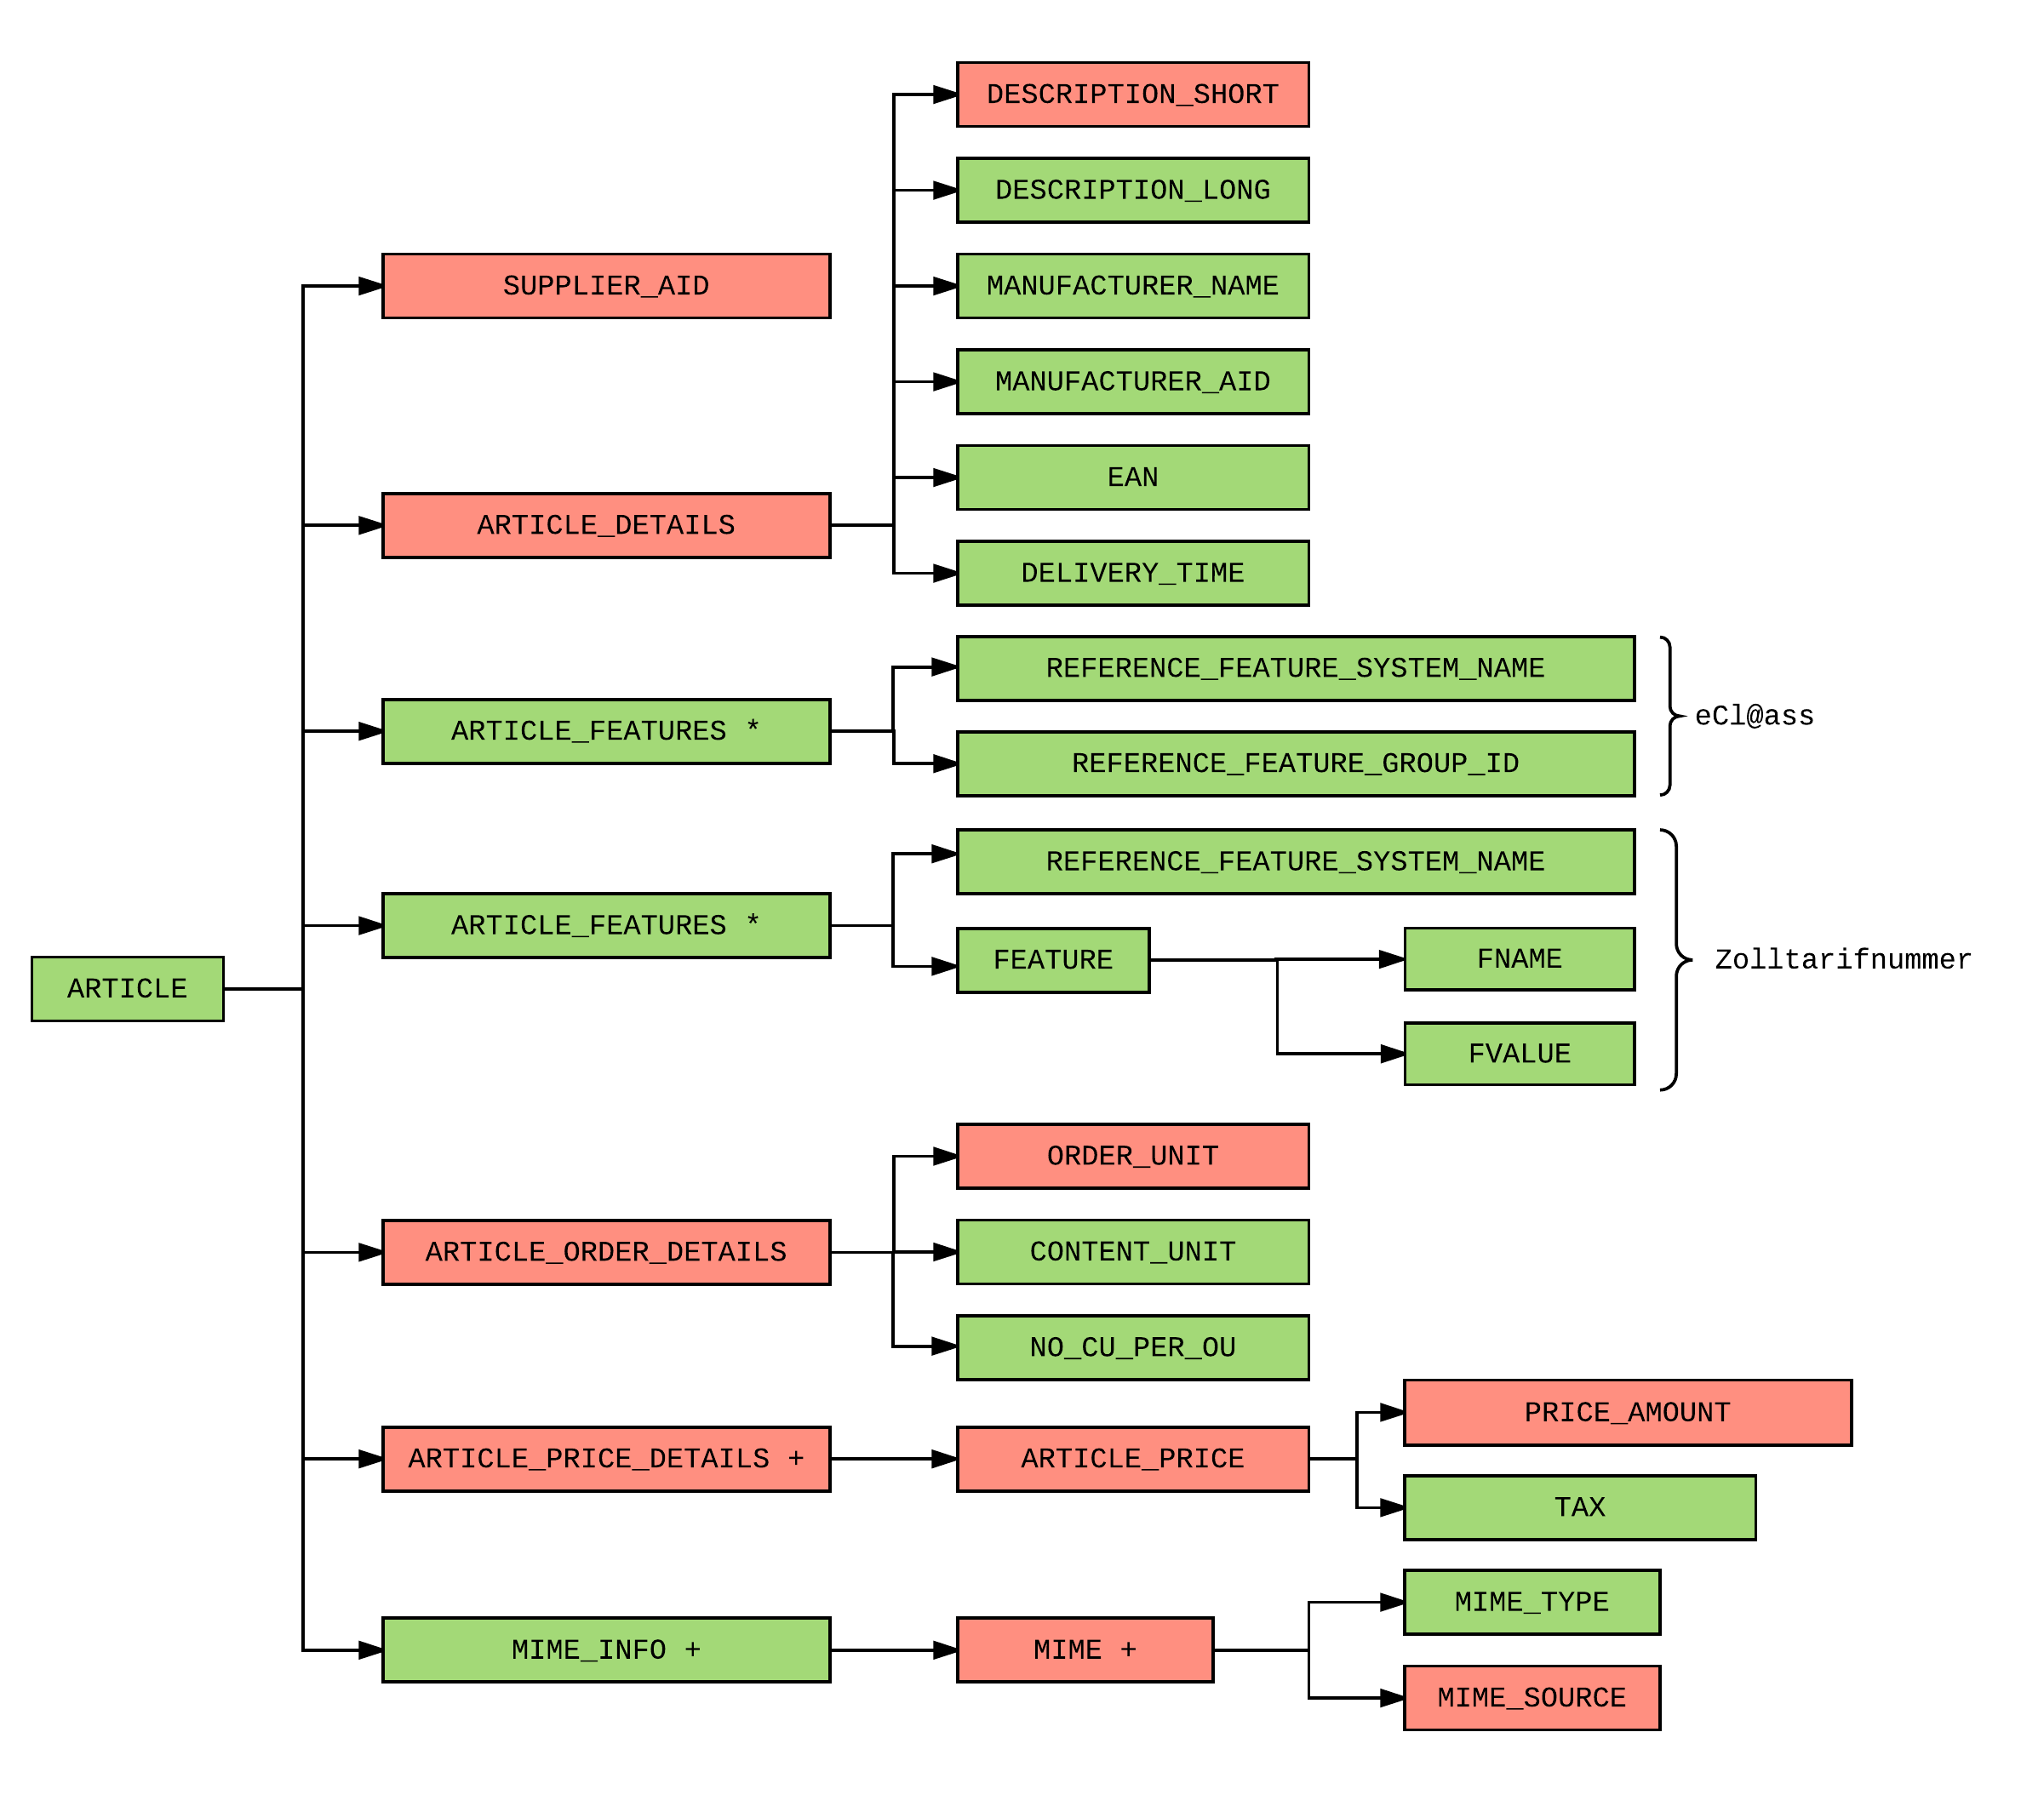
\includegraphics[width=1\linewidth]{img/Article}
		\captionof{figure}[Article]{Article}
		\label{fig:header}
		\vspace{1em}
	\end{minipage}
	
	Das Element \texttt{ARTICLE} verfügt über das Attribut \texttt{mode}, welches Informationen darüber enthält, ob es sich um die Anlage eines neuen Artikel, ein Update der Artikelinformationen oder die Löschung eines Artikels handelt.
	
	\begin{lstlisting}
	<ARTICLE mode="new">...</ARTICLE>
	<ARTICLE mode="update">...</ARTICLE>
	<ARTICLE mode="delete">...</ARTICLE>
	\end{lstlisting}
	\pagebreak
	
	
	\textbf{\underline{Das Element ARTICLE\_TO\_CATALOG\_GROUP\_MAP}}\\
	
	Um Produkte ihren Kategorien zuordnen zu können wird das Element \texttt{ARTICLE\_TO\_CATALOGGROUP\_MAP} verwandt. Es erfolgt hier eine Verknüfung aus der eindeutigen Artikelnummer und der \texttt{GROUP\_ID} welcher der Artikel zugeordnet werden soll. Eine Mehrfachzuordnung ist möglich, d.h. ein Artikel kann in unterschiedliche Kategorien \enquote{eingehängt} werden.
	
	\begin{minipage}{\linewidth}
		\vspace{1em}
		\centering
		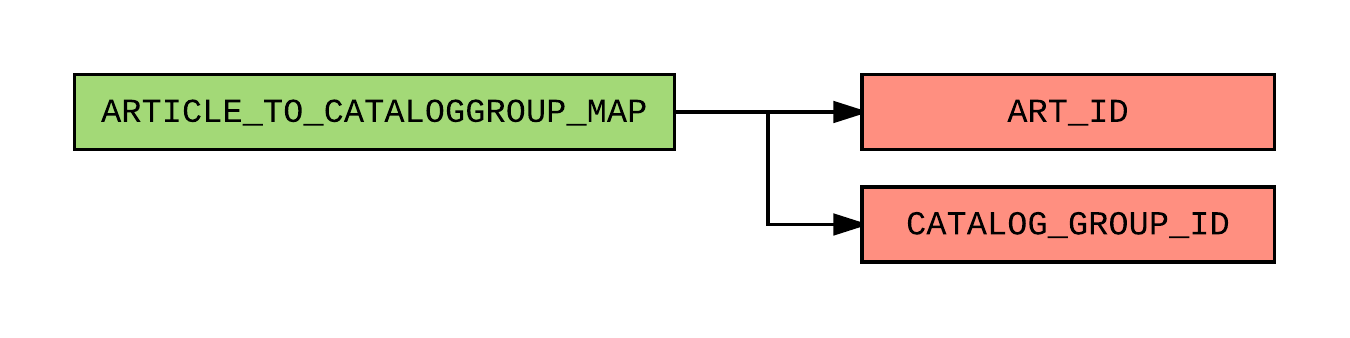
\includegraphics[width=0.7\linewidth]{img/articleGroupMap}
		\captionof{figure}[ArticleGroupMap]{ARTICLE\_TO\_CATALOG\_GROUP\_MAP}
		\label{fig:header}
		\vspace{1em}
	\end{minipage}
	
	Im Kontext der Transaktion \texttt{T\_UPDATE\_PRODUCTS} verfügt das Element zusätzlich über das Attribut \texttt{mode}, mit welchem angegeben wird, ob es sich um eine Neuzuweisung zu einer Kategorie handelt oder der Artikel aus einer Kategorie entfernt werden soll.
	
	\begin{lstlisting}
	<ARTICLE_TO_CATALOGGROUP_MAP mode="new">...</<ARTICLE_TO_CATALOGGROUP_MAP>
	<ARTICLE_TO_CATALOGGROUP_MAP mode="delete">...</<ARTICLE_TO_CATALOGGROUP_MAP>
	\end{lstlisting}
	
	
	\textbf{\underline{Zusammenspiel verschiedener Transaktionen}}\\
	
	Die folgende Grafik zeigt, wie das empfangende System bei der Transaktion \texttt{T\_NEW\_CATALOG} je nach übergebener \texttt{CATALOG\_ID}, \texttt{CATALOG\_VERSION} und \texttt{LANGUAGE} reagiert.
	
	\begin{minipage}{\linewidth}
		\vspace{1em}
		\centering
		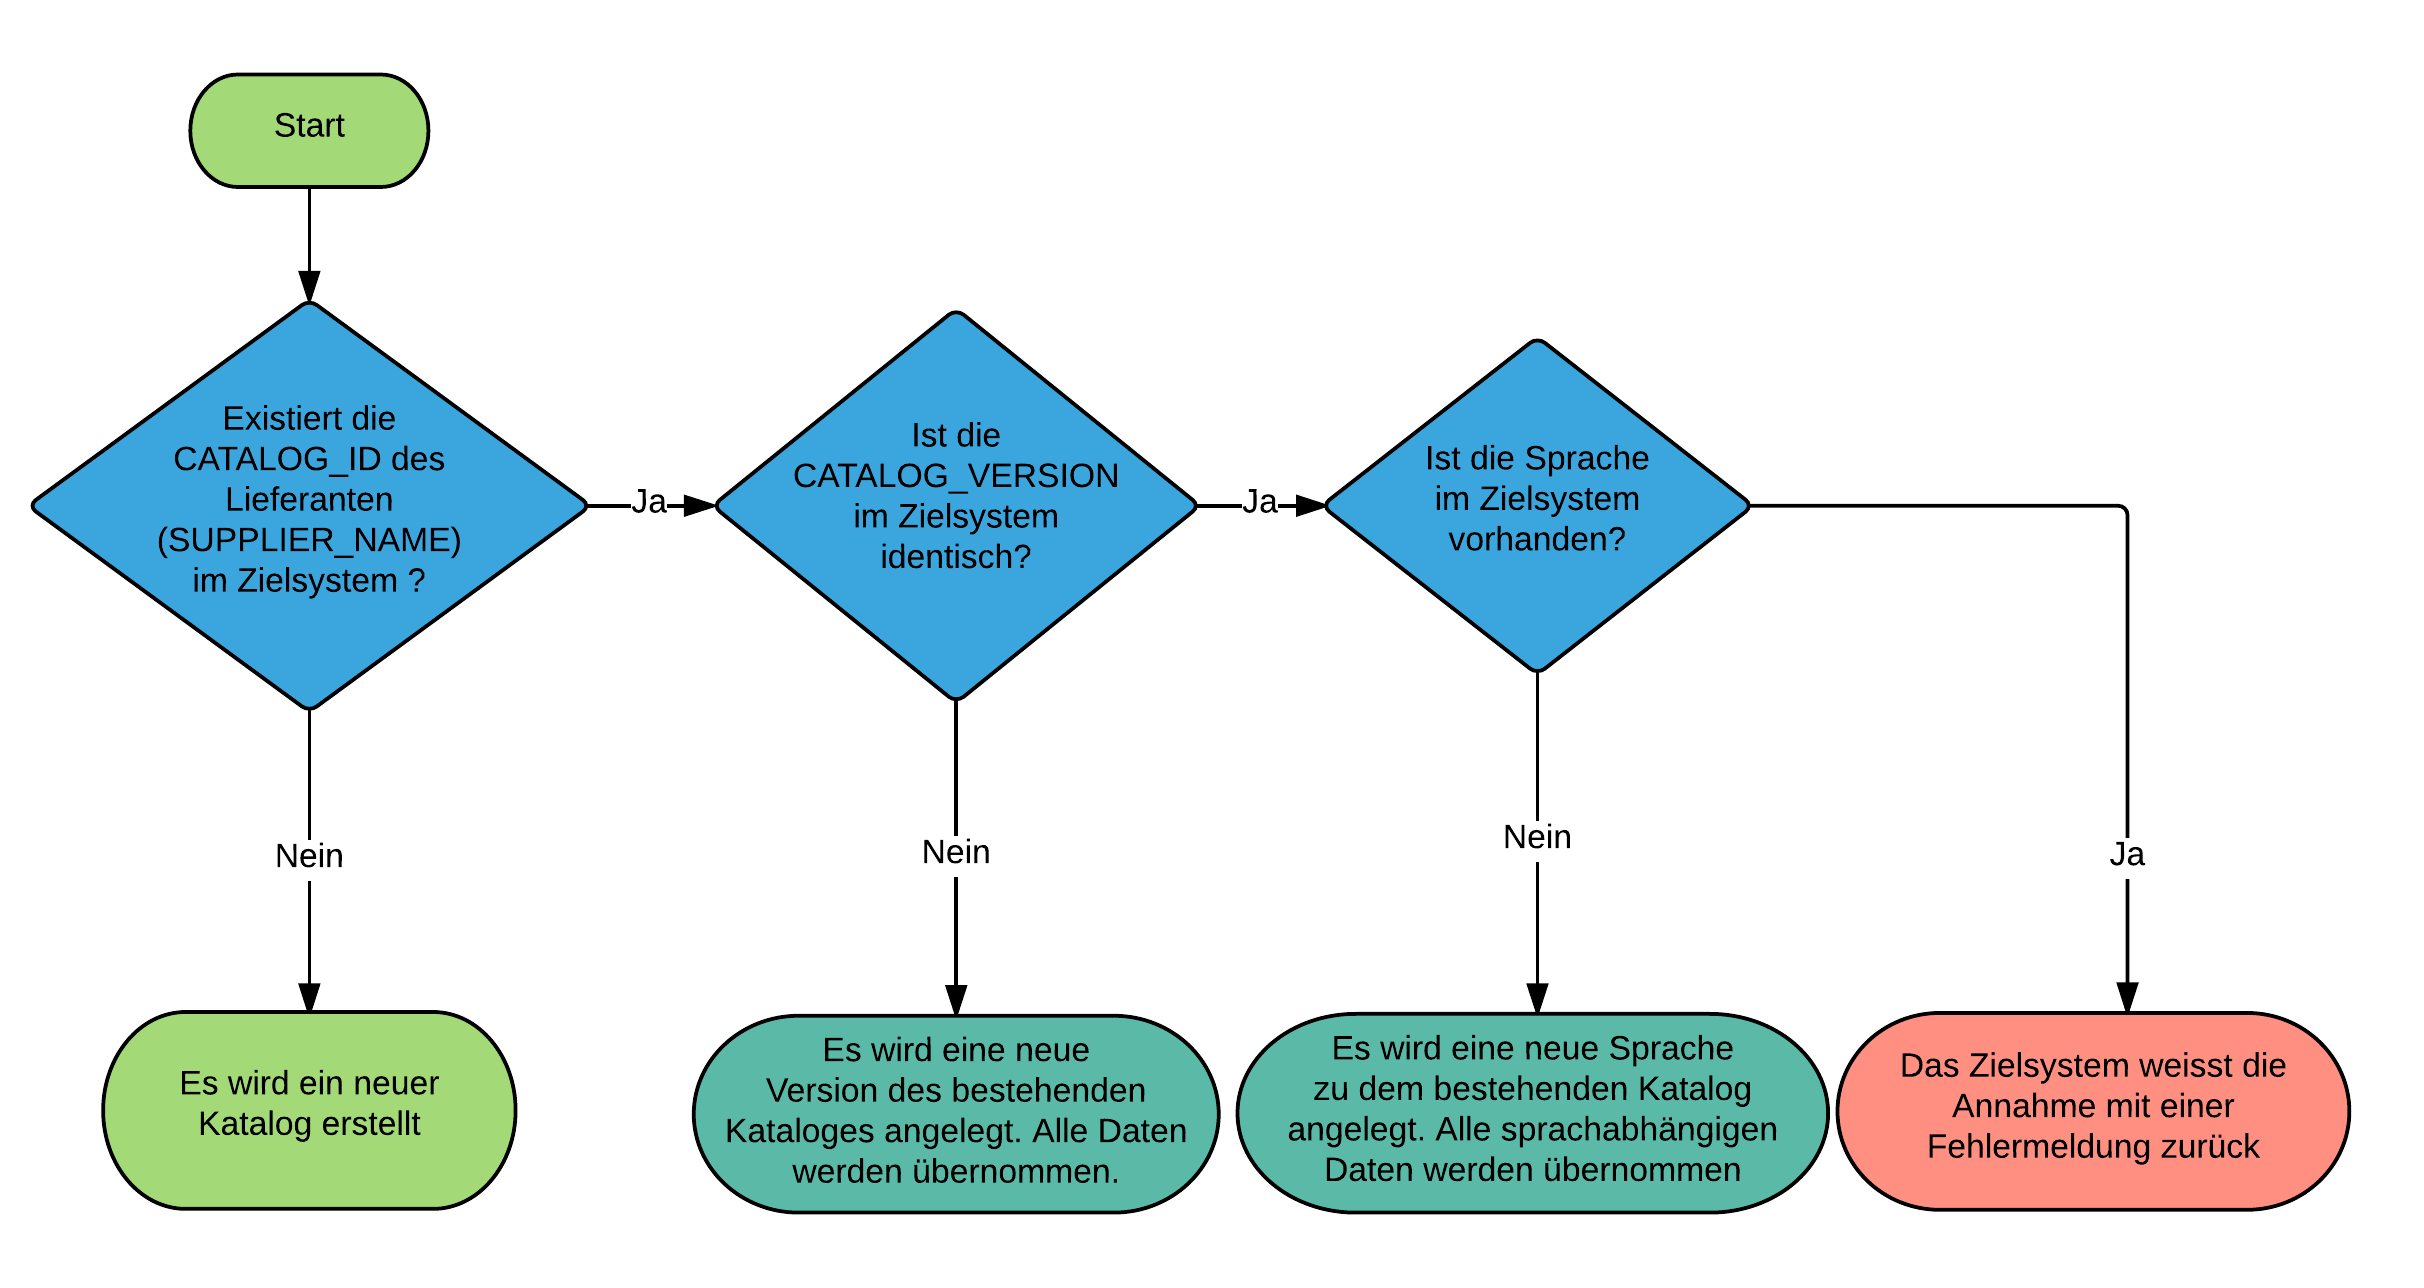
\includegraphics[width=0.8\linewidth]{img/newCatalogLogik}
		\captionof{figure}[New Catalog Logik]{Logik des empfangenden Systems bei der Transaktion  \texttt{T\_NEW\_CATALOG}}
		\label{fig:header}
		\vspace{1em}
	\end{minipage}
	
	Kommt die Transaktion \texttt{T\_UPDATE\_PRODUCTS} zur Anwendung, gilt es folgendes zu beachten\footnote{vgl. hierzu: BMECat V 1.2 Spezifikation, Seite 52}: 
	\begin{itemize}
		\item Die übertragene \texttt{CATALOG\_ID} des jeweiligen Lieferanten und die dazugehörige\\ \texttt{CATALOG\_VERSION} müssen im Zielsystem bereits vorhanden sein.
		\item Das Attribut \texttt{prev\_version} muss bei der ersten anderen Transaktionsart nach\\ \texttt{T\_NEW\_CATALOG}, (\texttt{T\_UPDATE\_PRODUCTS},\texttt{T\_UPDATE\_PRICES}) auf \enquote{0} gesetzt werden.
		\item Danach wird es bei jeder solchen Transaktion um \enquote{1} erhöht.
	\end{itemize}
	
	
	---- Übersicht, tabellarisch oder nicht über die wichtigsten Felder und ihre Einschränkungen, vor allem die von Mercateo ----
	
	\subsection{Das Cake-PHP Framework}
	
	Cake PHP ist ein Webframework, das dem MVC (Model-View-Controller) Schema folgt und dabei die Softwaredesignparadigmen DRY (Don't repeat yourself) und \enquote{Convention over configuration} umsetzt. 
	
	\subsubsection{Convention over Configuration in CakePHP}
	
	%Hier noch eine Erklärung zu COC von den Big Five einfügen
	In CakePHP wird das Softwaredesign-Paradigma der \enquote{Konvention vor Konfiguration} konsequent umgesetzt.\newline % Entweder duetsch oder englisch bzw erläuternd übersetzen
	
	 Die Klassennamen von \textbf{Controllern} sind im Plural verfasst, \enquote{CamelCased} und enden auf \textit{Controller}. \texttt{UsersController} und \texttt{ArticleCategoriesController} sind Beispiele dafür. Eine öffentliche Methode eines solchen Controllers kann über einen Webbrowser aufgerufen werden. Per Konvention werden Controllernamen in URLs klein geschrieben und mit Bindestrich verbunden.
	\url{http://samplesite.com/article-categorie/view} ruft demnach die öffentliche \texttt{view()} Methode des ArticleCategoriesControllers auf.\\
	\newline
	Die Namen von \textbf{Model} Klassen sind \enquote{CamelCased} und im Plural. Der Name der zum Model gehörenden Tabelle ist im Plural verfasst und mit einem Unterstrich verbunden.\\
	\texttt{article\_categories} ist die dem Model \texttt{ArticleCategories} zugrundeliegende Tabelle. Um einen Fremdschlüssel auf eine Tabelle zu vergeben genügt es das Suffix \texttt{\_id} an den kleingeschriebenen Namen dieser Tabelle anzuhängen. Wenn Users eine hasMany Beziehung zu Articles hat, kann mit dem Fremdschlüssel \texttt{user\_id} in der \texttt{articles}-Tabelle auf den entsprechenden Eintrag in der \texttt{users}-Tabelle verwiesen werden. \newline
	
	Die Template Datei einer \textbf{View} ist nach der entsprechenden Methode im Controller benannt, die sie darstellen soll. Die \texttt{view()} Methode der \texttt{ArticlesController} Klasse würde demnach unter \texttt{src/Template/Articles/view.ctp} nach einem View-Template suchen\footnote{vgl. hierzu: \url{http://book.cakephp.org/3.0/en/intro/conventions.html}}.
	
	\subsubsection{Model}
	
	Das Backend einer CakePHP Anwendung wird von einer SQL Datenbank gebildet. Das Model repräsentiert die Daten einer Anwendung und enthält die Geschäftslogik zur Datenmanipulation. Nach der CakePHP Konvention wird die Datenbankverbindung einmal in der Daeti \texttt{config/app.php} konfiguriert. Die Model-Klasse stellt dabei Methoden zur Verfügung, über die es möglich ist, den Zustand der Daten abzufragen, die Daten zu filtern und zu verändern. Die CRUD-Funktionalität (CREATE-READ-UPDATE-DELETE) ist so direkt im Model integriert.\footnote{vgl. hierzu: Webentwicklung mit CakePHP, 2. Auflage, O'Reilly, Seite 7}. 
	Die Beziehungen einzelner Models zueinander werden über \textit{Associations} hergestellt. Die vier Assoziationstypen in CakePHP sind:\\

	\begin{table}[!htbp]
		\begin{tabularx}{\textwidth}{p{1cm} X X p{8cm}}
			\cline{2-4}
			\rowcolor[HTML]{EFEFEF} 
			 Nr. & Beziehung & Typ & Beispiel \\ \cline{1-4} \addlinespace
			1 & one to one & hasOne & Ein Museum hat eine Adresse. \\
			2 & one to many & hasMany & In einem Museum hängen mehrere Kunstwerke. \\
			3 & many to one & belongsTo & Mehrere Bilder gehören zu einem Museum. \\  
			4 & many to many & belongsToMany & Ein Student hat mehrere Professoren. Ein Professor hat mehrere Hörer. \\ \addlinespace \cline{1-4}     
		\end{tabularx}
		\captionbelow{Übersicht der Assoziationstypen in CakePHP}
	\end{table}
		
	
	
	
	Es ist möglich ein \textit{Model} um ein oder mehrere \textit{Behavior} zu erweitern. Dabei handelt es sich um Klassen, in denen, ähnlich einem Trait, Funktionen zur Erweiterung des Models gekapselt sind. Ein Beispiel hierfür ist das Tree-Behavior, das es ermöglicht hierarchische Datenstrukturen in der Datenbank zu pflegen. Anwendung hierfür kann z.B. die Abbildung einer Kategoriestruktur sein \footnote{vgl. hierzu: \url{http://book.cakephp.org/3.0/en/orm/behaviors/tree.html}}.
	
	Mit Hilfe von im Model definierten Validatoren können zu speichernde Daten auf Vollständigkeit und Konsistenz geprüft werden. 

	\lstset{language=PHP}
	\begin{lstlisting}

	$validator
     	->requirePresence('catalog_name', 'create')
     	->notEmpty('catalog_name')
     	->add('catalog_name', [
	         'maxLength' => [
	             'rule' => ['maxLength', 100],
	             'message' => 'maxLength = 100.'
	         ]
     ]);
	
	\end{lstlisting}
	
	\subsubsection{View}
	
	Die View ist für die Darstellung der Daten in der Anwendung zuständig. Eine View ist in CakePHP immer auf einen bestimmten Controller bezogen und wird nicht für die Darstellung anderer Daten verwendet\footnote{vgl. hierzu: Webentwicklung mit CakePHP, 2. Auflage, O'Reilly, Seite 7}. CakePHP View Template Dateien Enden auf \enquote{.ctp} und bedienen sich der alternativen PHP Syntax für Kontrollstrukturen und Ausgabe. 
	In einer View kann direkt auf Variablen zugegriffen werden die in der entsprechenden Controller Methode gesetzt wurden:\\ 
   \lstset{language=PHP} 
	\begin{lstlisting}
	$this->set('articleCategories',  $articleCategories);
	\end{lstlisting}
	  Die Codebeispiele zeigen, wie die Variable \texttt{\$articleCategories} im Controller für die View freigegeben wird und dort z.B. mit einer foreach-Schleife durchlaufen werden kann um ihren Inhalt auszugeben. 
		\lstset{language=PHP}
		\begin{lstlisting}[caption={Alternative PHP Syntax}] 	
		<ul>
	   	<?php foreach ($todo as $item): ?>
		  <li><?= $item ?></li>
		<?php endforeach; ?>
		</ul>
		\end{lstlisting}
	 Eine View ist dabei nicht auf das Anzeigen von HTML Inhalten beschränkt, sondern kann auch dazu verwandt werden XML- oder JSON- Repräsentationen der angefragten Daten zurückzuliefern.
	\subsubsection{Controller}
	Der Controller regelt den Ablauf der Benutzerinteraktion.
	Er ist dafür zuständig, dass das richtige Model aufgerufen und die entsprechende Antwort oder View erzeugt wird. Er dient dabei als eine Art Vermittler zwischen dem Model und der View. Normalerweise ist in CakePHP ein Controller für ein Model verantwortlich, es ist dennoch möglich, oft auch nötig, dass ein Controller mit mehreren Models arbeitet.
	
	Der Controller enthält eine Reihe von  Methoden die HTTP Anfragen verarbeiten. Diese Methoden werden in CakePHP \textit{actions} genannt. Per Definition ist jede öffenliche Methode in einem Controller eine \textit{action} und über eine URL der Form \url{http://samplesite.com/article-categorie/view} erreichbar.
	Eine \textit{action} ist für die Verarbeitung der Anfrage und das Zurückliefern einer Antwort zuständig. Im Normalfall wird dabei eine View erzeugt, es können aber auch (wie im Abschnitt Model erläutert) XML oder JSON Daten zurückgeliefert werden.\footnote{vgl. hierzu: \url{http://book.cakephp.org/3.0/en/controllers.html}}
	
	\subsubsection{Component}
	Komponenten (Components) sind in sich geschlossene Bereiche innerhalb einer Applikation, die eine bestimmte Funktionalität kapseln und über die Grenzen eines Controllers hinaus verfügbar machen. Sollen bestimmte logische Prozesse in verschiedenen Teilen einer Anwendung zur Verfügung stehen - insbesondere in unterschiedlichen Controllern- so ist es sinnvoll diese in eine Komponente auszulagern\footnote{vgl. hierzu: Webentwicklung mit CakePHP, 2. Auflage, O'Reilly, Seite 223}.
	Die Möglichkeit mit Komponenten zu arbeiten setzt das DRY Paradigma konsequent um.
	
	\subsubsection{Shell}	%Übergang zwischen Shell und Baking flüssiger gestalten
	CakePHP bietet die Möglichkeit Konsolenanwendungen zu schreiben. Dies ist nützlich für Anwendungen die per Cronjob ausgeführt werden sollen oder für solche die nicht aus einem Browser erreicht werden müssen bzw. sollen\footnote{vgl. hierzu \url{http://book.cakephp.org/3.0/en/console-and-shells.html}}. 
	Eine der wichtigsten Funktionalität der Cake Shell ist das \enquote{Backen} (Baking). Gemeint ist damit die automatische Generierung von Code. Der Befehl \texttt{bin/cake bake} erstellt, je nach gewählter Option, ganze MVC Grundgerüste, Controller- oder Model- Klassen, Plugin Verzeichnisstrukturen oder Shell-Klassen. Einzelne Funktionalitäten einer Shell Klasse können in Tasks ausgelagert werden.  
	
	
	\section{Analyse der Aufgabe und der Anforderungen}
	
	\subsection{Funktionale und nichtfunktionale Anforderungen}	
		
		\subsubsection{Funktionale Anforderungen}
		\begin{enumerate}[noitemsep]
		\item Die in iTool hinterlegten Produkt- und Herstellerdaten sollen in das BMECat Format in der Version 1.2 überführt werden. 
		\item Es sollen die beiden Transaktionsarten \texttt{T\_NEW\_CATALOG} und \texttt{T\_UPDATE\_PRODUCTS} umgesetzt werden\footnote{vgl. dazu: Kapitel 1.2.2 \& 1.2.3}.
		\item Die Produktkategoriestruktur des iTool soll in das Kataloggruppensystem des BMECat überführt werden.
		\item Die Katalogerstellung soll in einer CakeShell erfolgen.
		\item Das Programm soll über einen CronJob gesteuert werden können.
		\item Es soll Mercateo ermöglicht werden Bestandsdaten zu den im Katalog vorhanden Produkten über einen Webservice abzurufen. Der Aufruf erfolgt über eine URL der Form \url{http://itool.local/mercateo/availability/12}, wobei der letzte Wert die angefragte SKU repräsentiert. 
		\item Es sollen Kataloge für unterschiedliche Verkäufer erstellt werden können.
		\item Die zu exportierenden Produkte sollen in einer Warteschlange gehalten werden um die verschiedenen Artikelmodi (\enquote{new}, \enquote{update}, \enquote{delete}) ausgezeichnet werden zu können.
		\item Dem Dokumentennamen sollen der Name des Verkäufers sowie Datum und Uhrzeit der Entstehung entnommen werden können.
		
		\end{enumerate}
		\subsubsection{Nichtfunktionale Anforderungen}
		\begin{enumerate}[noitemsep]
		\item Das Katalogdokument soll gültig sein.\\ Das bedeutet, dass es fehlerfrei gegen das entsprechende XSD Schema laufen kann.
		\item Das Katalogdokument soll vollständig sein. \\Das bedeutet, es müssen zum einen mindestens jene Felder im BMECat Dokument vorkommen, die die BMECat Spezifikation verlangt. Zusätzlich müssen jene Felder vorkommen, die die Mercateo Spezifikation erfordert und zwar unter zusätzlicher Beachtung der Limitierungen bzw. Besonderheiten jener Spezifikation. 	
		\item Die zu exportierenden Produktdaten sollen über das GUI des iTool editier- und einsehbar sein.
		\item Die Verkäufer- und Katalogspezifischen Daten sollen über das GUI des iTool editier- und einsehbar sein. 
			\begin{itemize}[noitemsep]
			\item Verkäuferspezifische Daten sind:
				\begin{itemize}[noitemsep]
					\item \texttt{core\_seller\_id}
					\item \texttt{core\_marketplace\_id} 
					\item \texttt{core\_currency\_id} 				
				\end{itemize}
			\item Katalogspezifische Daten sind (in Klammern steht das entsprechende BMECat Element):
				\begin{itemize}[noitemsep]
					\item Der Name des verkaufenden Unternehmens (\texttt{SUPPLIER\_NAME})
					\item Der Titel des Kataloges (\texttt{CATALOG\_ID})
					\item Die Katalogversion (\texttt{CATALOG\_VERSION})	
					\item Die Kennung des Kataloggruppensystems (\texttt{GROUP\_SYSTEM\_ID})	
					\item Der Name des Kataloggruppensystems (\texttt{GROUP\_SYSTEM\_NAME})	
					\item Die Beschreibung des Kataloggruppensystems (\texttt{GROUP\_SYSTEM\_DESCRIPTION})			
				\end{itemize}
			\end{itemize}
		\item Der Entwurf soll den Designprinzipien der \enquote{Single Responsibility} und des \enquote{Open Closed} folgen.
		\item Die zu exportierenden Daten sollen möglichst schon vor dem Export in das BMECat-Format validiert werden.
		\item Es sollen zumindest \enquote{Single-Products} gelistet werden können.
		\item Es sollen nach Möglichkeit auch \enquote{Configurable-Products} gelistet werden können.
		\item Es soll eine große Anzahl (\textgreater 10.000) an Produkten ohne Speicherüberläufe exportiert werden können.
	%	\item Die Software soll auf einem Apache2 Webserver unter Linux lauffähig sein.
		\end{enumerate}
				 

		
		\subsection{Zielstellung}
		
		Ziel der prototypischen Entwicklung der Software ist es, zu zeigen, dass die in iTool gehaltenen Produktdaten in das BMECat-Format überführt werden können. Es soll insbesondere sichergestellt werden, dass die erstellten Katalogdokumente fehlerfrei gegen die enstprechenden XSD-Schemata laufen. Falls Fehler auftreten, sollen diese geloggt werden. Da mit einer großen Anzahl zu exportierende Produkte zu rechnen ist, muss verantwortungsvoll mit den zur Verfügung stehenden Ressourcen umgegangen werden. Es sollen zunächst nur 'Simple-Products' exportiert werden. Die Verwaltung der Produkt-, Katalog- und Herstellerdaten soll einfach, nachvollziehbar und komfortabel sein. Die erwähnten Designprinzipien sollen, aufgrund der daraus resultierenden besseren Wartbarkeit des Codes, umgesetzt werden.
		

				
%		\subsection{Informelle Aufgabenbeschreibung}
%		Ziel der Arbeit ist es die von der Software iTool aus verwaltbaren, in verschiedenen Tabellen einer SQL-Datenbank gehaltenen Produkt-, Katalog- Kategorie- und Herstellerdaten in ein von Mercateo verarbeitbares Format (dem BMECat) zu bringen. Dabei gilt es, den Anforderderungen der Spezifikationen sowohl das BMECat, als auch der besonderen Anforderungen seitens Mercateo zu genügen.
%		Es soll möglich sein, die erwähnten Daten aus dem UI des iTool heraus nach dem CRUD-Prinzip zu bearbeiten. 
%		Die eigentliche Erstellung der unterschiedlichen Kataloge (neuer Katalog bzw. Produktupdatekatalog) erfolgt dabei (automatisiert) über die CakePHP Shell. Kataloge können dabei für unterschiedliche Verkäufer erstellt werden.
%		Zudem soll es Meracteo ermöglicht werden Bestandsdaten zu einer bestimmten Artikelnummer über ein Webinterface abzurufen.
		

		

	
	\subsection{Einschätzung der verwendeten Technologien}

	
	\subsubsection{BMECat Format}
	
	Allgemeine Vorteile die sich aus dem XML-Format ergeben sind die gleichzeitige Mensch- und Maschinenlesbarkeit sowie die Möglichkeit das Dokument gegen ein XML-Schema testen zu können. So kann schon direkt nach der Erzeugung des BMECat Dokumentes überprüft werden, ob die geschriebenen Elemente vom richtigen Datentyp sind und das Dokument der in der XSD Datei festgelegten Struktur folgt. Weitere Vorteile speziell des BMECat Standards sind\footnote{vgl. hierzu: \url{http://wiki.prozeus.de/index.php/BMEcat}}:
	
	\begin{itemize}[noitemsep]
	\item konfigurierbare Produkte sind abbildbar.
	\item mehrsprachige Kataloge sind in einem Katalogdokument abbildbar.
	\item Übermittlung multimedialer Datenelemente ist möglich (z.B. Produktvideos).
	\item gilt zumindest in Deutschland als etabliertes Katalogaustauschformat.
	\end{itemize}
	
	
	
	\subsubsection{Datenübertragung zu Mercateo}
	
	Die Übertragung der Katalogdatei zum Mercateo-Server geschieht über FTP. Neue Dateien werden alle 30 Minuten vom Mercateo-System verarbeitet.\\
	\textbf{Vorteile:}
 	\begin{itemize}[noitemsep]
   	\item einfach anzuwenden.
   	\item Eine korrekte Datenübertragung ist durch die Fehlerbehandlung von TCP gewährleistet.
   	\end{itemize}
	\textbf{Nachteile:}
   	\begin{itemize}[noitemsep]
   	\item Datenübertragung nicht nach außen abgesichert.
   	\item Übertragene Daten können mitgelesen und manipuliert werden.
   	\item Benutzerkennung und Passwort können abgefangen werden
   	\item Die vollständige Datenübertragung kann nicht garantiert werden (fehlende Prüfsummen o.ä.)
   	\end{itemize}
   	\textbf{Fazit:}\\
	Nicht optimal, vor allem aus Sicherheitsgründen. Zudem Fehleranfällig, wenn die Ordnerstruktur- und Dateinamenskonventionen von Mercateo nicht eingehalten werden \footnote{vgl. hierzu: \url{http://www.mercateo.com/support/verkaufen/katalog-allgemeine-informationen/datenuebertragung-per-ftp/}}.

	\pagebreak	
	\section{Entwurf}
	
	Bei dem Entwurf der Software sollen die Prinzipien der \textit{Single-Responsibility} und des \textit{Open-Closed} zur Anwendung kommen.
	
	\begin{itemize}
	\item \textbf{Das Single-Responsibility-Prinzip}\\besagt, dass eine Klasse nur eine fest definierte Aufgabe hat und nur Methoden enthält, die zur Erfüllung dieser Aufgabe notwendig sind.
	\item \textbf{Das Open-Closed-Prinzip}\\ besagt, dass Klassen sowohl offen für Erweiterungen, als auch geschlossen für Modifikationen seien sollen. Das Prinzip der Vererbung (Polymorphie) setzt dies um.
	\end{itemize}
	
	\subsection{Katalogerstellung}
	
	Die Erstellung der BMECat Dokumente wird über eine CakePHP Shell und von dort aus aufrufbare Tasks realisiert. Das hat den Vorteil, dass diese, im Bedarfsfall, über einen Cronjob automatisiert werden können.
	Die Logik zur Erstellung eines neuen BMECat Dokumentes wird in die Klasse \texttt{AddNewCatalogTask} ausgelagert, die zur Erstellung eines Updatekataloges in die Klasse 
	\texttt{UpdateCatalogTask}. Mit der Klasse \texttt{DeleteCatalogTask} wird das Löschen von den zu exportierenden Katalogdaten umgesetzt. Das Schreiben eines Katalogdokumentes wird durch die Componentklasse \texttt{BMECatComponent} realisiert, die sich wiederum der Komponentenklasse \texttt{XMLWriterComponent} bedient. Hier kommt das \textit{Single-Responsibility} Prinzip zur Anwendung; Jede Klasse erfüllt genau eine Aufgabe. \texttt{AddNewCatalogTask}, \texttt{UpdateCatalogTask} und \texttt{DeleteCatalogTask} werden von der Basisklasse \texttt{CatalogToolsTask} abgeleitet. So wird das Prinzip des \textit{Open-Closed} umgesetzt.

	\begin{minipage}{\linewidth}
		\vspace{1em}
		\centering
		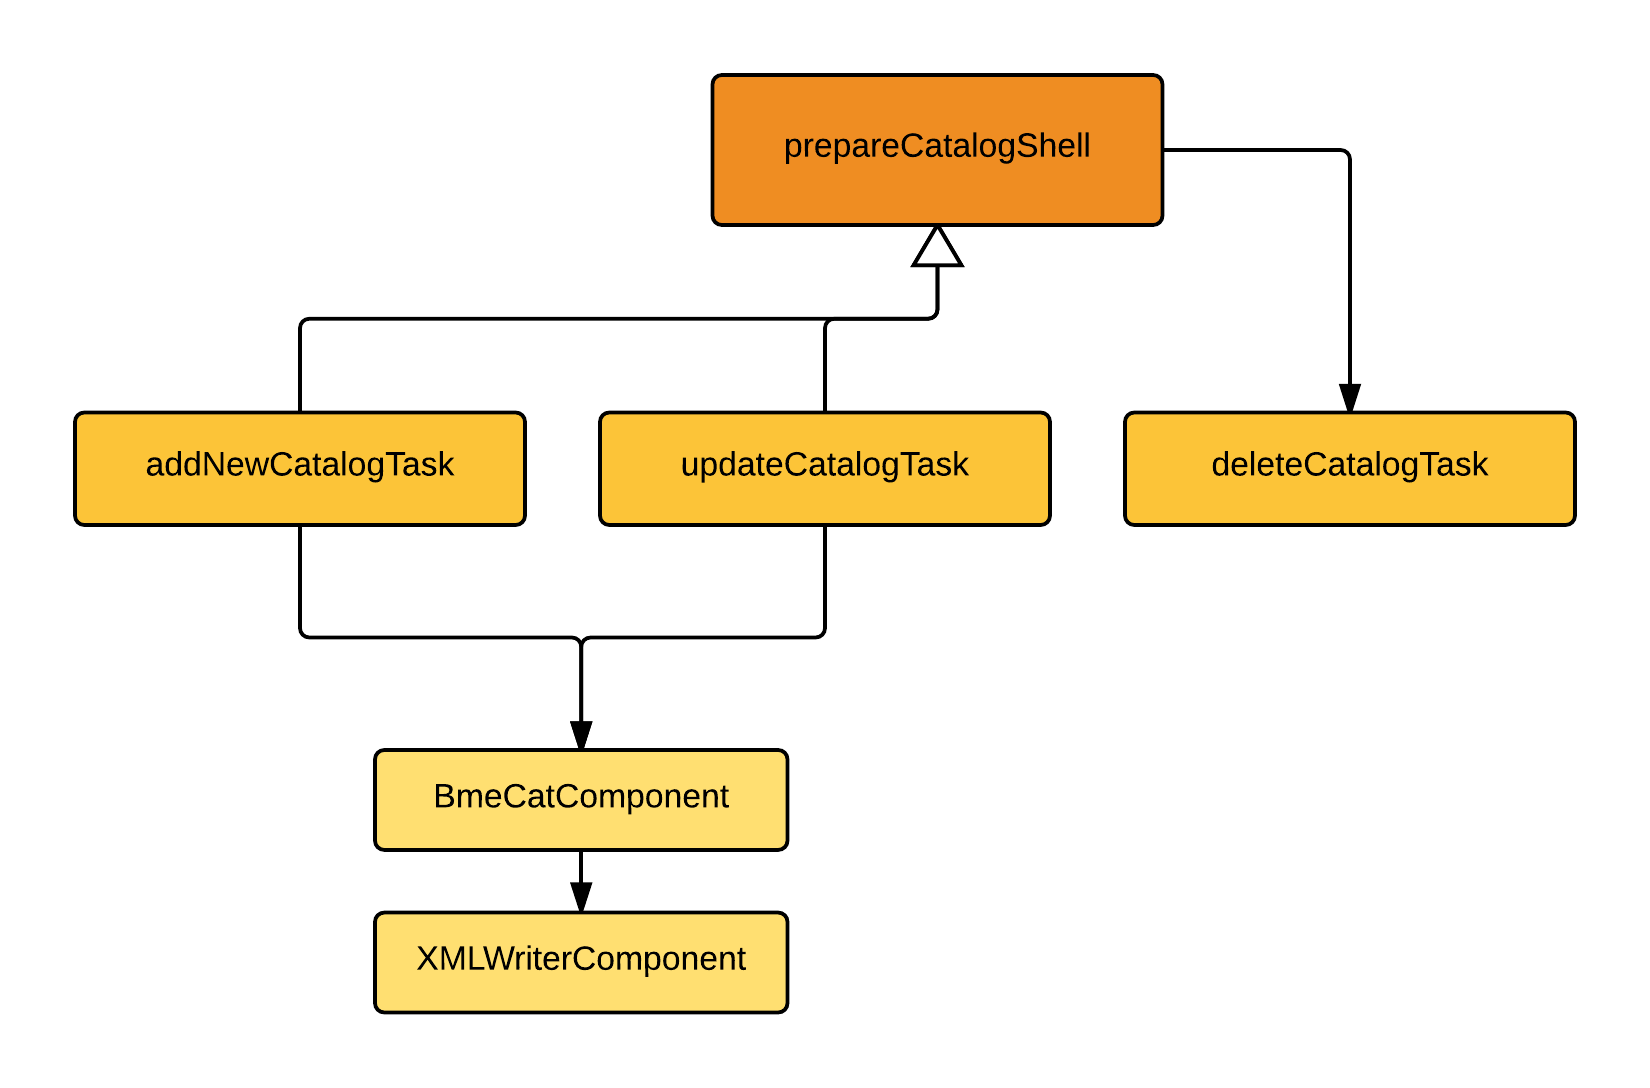
\includegraphics[width=0.7 \linewidth]{img/VererbungShellSimple}
		\captionof{figure}[BasicLogic]{Vererbungshierarchie der Task-Klassen}
		\vspace{1em}
	\end{minipage}	
	
	Es soll möglich sein beim Aufruf des Tasks die \textit{id} des \texttt{core\_sellers} zu übergeben, dessen Produkte exportiert werden sollen. Die Spezifikation des BMECat verlangt, dass im Katalogdokument bestimmte Informationen zur Katalogversion, dem Katalognamen, der der Preisauszeichnung zu Grunde liegenden Währung \textit{etc.} aufgeführt werden. Diese Daten werden in der Tabelle \texttt{mercateo\_accounts} gespeichert und können über die GUI des iTool eingesehen, erstellt, gelöscht und geändert werden.\\
	
	\begin{minipage}{\linewidth}
		\vspace{1em}
		\centering
		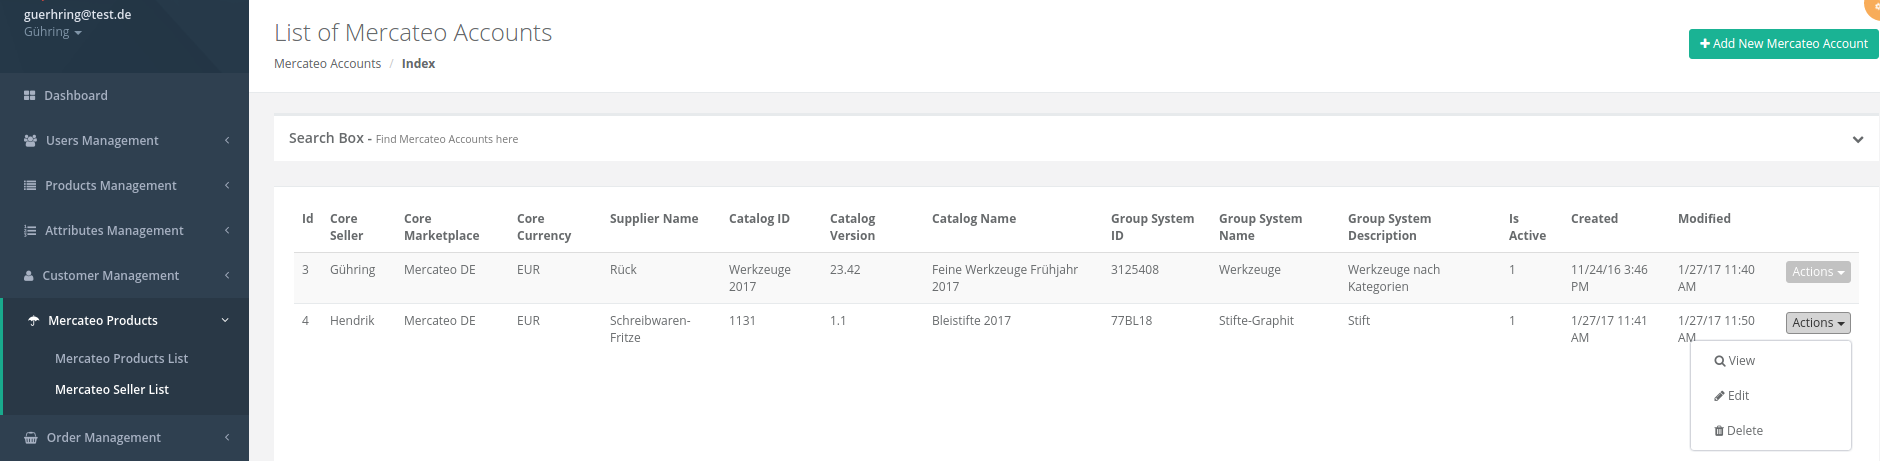
\includegraphics[width=1 \linewidth]{img/iToolSeller}
		\captionof{figure}[BasicLogic]{Abbildung der \texttt{mercateo\_accounts} Daten im iTool}
		\vspace{1em}
	\end{minipage}
	
	 Der Zeitpunkt der Katalogerstellung sowie dessen fortlaufende Versionsnummer (das Attribut \texttt{prev\_version}) werden in die bereits im iTool vorhandene Tabelle \texttt{core\_configurations} geschrieben. Zur Zwischenspeicherung der zu exportierenden Daten kommt die Tabelle \texttt{mercateo\_products} zum Einsatz. Die eigentlichen Produktdaten werde aus der Tabelle \texttt{core\_products} geladen, die Produktkategorien aus der mit dieser verknüpften Tabelle \texttt{core\_categories}. Mit Hilfe der Tabelle \texttt{core\_product\_updates} kann überprüft werden ob Artikeldaten aktualisiert wurde. Ist dem so, wird dort ein neuer Eintrag erstellt, der die \texttt{core\_product\_id} und den Zeitpunkt der Erzeugung enthält.
	

	
	
	\begin{table}[!htbp]
		\begin{tabularx}{\textwidth}{p{3.8cm} X  }
			\rowcolor[HTML]{EFEFEF} 
			Tabelle & Inhalt/Zweck  \\ \cline{1-2} \addlinespace[7pt]
			mercateo\_accounts & Speicherung statischer Daten wie Katalog- oder Herstellername. \\
			mercateo\_products & Zwischenspeicherung der zu exportierenden Daten.  \\
			core\_products & Hält sämtliche Produkdaten. \\
			core\_categories & Enthält Produktkategoriedaten. \\
			core\_configurations & Speichert Konfigurationsgruppen, Pfade und Werte. \\ 
			core\_product\_updates & Speichert den Timestamp der letzten Änderung eines \texttt{core\_products}. \\ \addlinespace[7pt] \cline{1-2} 	
	
		\end{tabularx}%
		\captionbelow{Übersicht der bei der Katalogerstellung verwendeten Tabellen}
	\end{table}
		
	\subsubsection{Die Tabelle \texttt{mercateo\_accounts}}
	
	Eine Übersicht der in \texttt{mercateo\_accounts} gespeicherten Werte bietet Tabelle 3. Wenn nicht anders angegeben entspricht das BMECat Element der Spaltenbezeichnung (\texttt{catalog\_id} $\approx$ \textless CATALOG\_ID\textgreater )

	\begin{table}[!htbp]
		\begin{tabularx}{\textwidth \small}{p{4cm} X p{2.8cm} }
			\rowcolor[HTML]{EFEFEF} 
			Spalte & Erläuterung & BMECat Element \\ \cline{1-3} \addlinespace[7pt]
			id & Primärschlüssel. & \multicolumn{1}{c}{\normalsize$\times$} \\
			core\_seller\_id & Fremdschlüssel auf \texttt{core\_sellers}.  & \multicolumn{1}{c}{\normalsize$\times$}  \\ 
			core\_marketplace\_id & Fremdschlüssel auf \texttt{core\_marketplaces}. & \multicolumn{1}{c}{\normalsize$\times$} \\ 
			core\_currency\_id & Fremdschlüssel auf \texttt{core\_currencies}.  &\multicolumn{1}{c}{ \textless CURRENCY\textgreater} \\ 
			supplier\_name & Name des verkaufenden Unternehmens. & \multicolumn{1}{c}{\normalsize \checked}   \\
			catalog\_id & Eindeutiger Bezeichner des Produktkataloges. & \multicolumn{1}{c}{\normalsize \checked}  \\
			catalog\_version & Version des Produktkataloges. & \multicolumn{1}{c}{\normalsize \checked} \\
			catalog\_name & Beliebiger Name, der den Produktkatalog beschreibt. & \multicolumn{1}{c}{\normalsize \checked} \\
			group\_system\_id & Kennung des Kataloggruppensystems. & \multicolumn{1}{c}{\normalsize \checked}  \\
			group\_system\_name & Name des Kataloggruppensystems. & \multicolumn{1}{c}{\normalsize \checked}  \\
			group\_system\_description & Beschreibung des Kataloggruppensystems. & \multicolumn{1}{c}{\normalsize \checked} \\	
			created & Timestamp, wann der Eintrag erzeugt wurde. & \multicolumn{1}{c}{\normalsize$\times$} \\
			modified & Timestamp, wann der Eintrag geändert wurde. & \multicolumn{1}{c}{\normalsize$\times$}\\\addlinespace[7pt] \cline{1-3} 
		\end{tabularx}%
		\captionbelow{Die Tabelle \texttt{mercateo\_accounts}}
	\end{table}
	Alle BMECat spezifischen Spalten werden über eine Methode im Model validiert, so dass nur Werte entsprechend der BMECat- bzw. Mercateo Spezifikationen gespeichert werden können.
	 
	\subsubsection{Die Tabelle \texttt{mercateo\_products}}

	Im Zentrum der Katalogerstellung steht die Tabelle mercateo\_products. Sie dient als Zwischenspeicher für die in \texttt{core\_products} hinterlegten Daten und gibt Auskunft darüber, ob (und wann) Produkte geändert, gelöscht oder neu hinzugefügt wurden. Dadurch wird sie zum zentralen Element zur Umsetzung der Transaktionen \texttt{T\_NEW\_CATALOG} und \texttt{T\_UPDATE\_PRODUCTS}. 
	
	\begin{table}[!htbp]
		\begin{tabularx}{\textwidth}{p{4cm} X}
		\rowcolor[HTML]{EFEFEF} 
		Spalte & Erläuterung \\ \cline{1-2} \addlinespace[7pt]
		id & Primärschlüssel \\
		core\_seller\_id & Die Id des Verkäufers \\
		core\_product\_id & Fremdschlüssel auf core\_products Tabelle \\
		core\_categorie\_id & Kategorie ID  \\
		status & Der Status des Eintrages \\
		sku & Die SKU des Artikels \\
		title & Die \enquote{DESCRITION\_SHORT} des Artikels  \\ 
		created & Timestamp, wann der Eintrag erzeugt wurde  \\
		modified & Timestamp, wann der Eintrag geändert wurde  \\\addlinespace[7pt] \cline{1-2} 
		\end{tabularx}%
		\captionbelow{Die Tabelle \texttt{mercateo\_products}}
	\end{table}
	
	Die Spalten \enquote{sku},\enquote{core\_category\_id} \& \enquote{title} sind notwendig um einen Artikel in einem BMECat Dokument als \textit{gelöscht} auszeichnen zu können. Die Spalte \enquote{status} akzeptiert vier  \textit{Zustände}: 
	

	\begin{tabularx}{\textwidth}{p{3cm} X}
	\rowcolor[HTML]{EFEFEF} 
	Zustand & Erläuterung \\ \cline{1-2} \addlinespace[7pt]
	\texttt{new} & Produktdaten wurden neu in \texttt{core\_products} angelegt. \\
	\texttt{update} & Produktdaten wurden geändert. \\
	\texttt{delete} & Produktdaten wurden aus \texttt{core\_products} gelöscht. \\
	\texttt{active} & Produktdaten wurden in das aktuelle BMECat Dokument übernommen. \\
	   \addlinespace[7pt] \cline{1-2} 
	\end{tabularx}%
		
	Diese Zustände sind die Werte die das Attribut \texttt{mode} des BMECat Elements \texttt{ARTICLE} annehmen kann. Gleichzeitig geben sie an dieser Stelle Auskunft darüber, ob ein in \texttt{core\_products} gespeicherter Datensatz neu ist bzw. gelöscht oder verändert wurde. Jene Datensätze die in das aktuelle BMECat Dokument geschrieben wurden, werden mit \enquote{active} markiert. Die in \texttt{mercateo\_products} gehaltenen Einträge können über das GUI manipuliert werden.
	
	\subsubsection{Allgemeiner Programmablauf bei der Katalogerzeugung}
	
	Wird die Shell unter Angabe des entsprechenden Tasks aufgerufen, wird zunächst überprüft ob der Nutzer die \textit{id} des Verkäufers angegeben hat, dessen Produkte exportiert werden sollen. Ist das nicht der Fall bricht das Programm mit einem Hinweis zum korrekten Aufruf ab. Falls die übergebene \textit{id} nicht in der Datenbank gefunden werden kann, so wird eine Liste aller verfügbaren Verkäufer ausgegeben. Anschließend wird, je nach gewähltem Task, ein initiales Katalogdokument oder ein Updatekatalogdokument erzeugt und im Anschluss daran mit dem entsprechenden XML Schema validiert. 
	
	\subsubsection{Katalogerstellungslogik in der Klasse \texttt{AddNewCatalogTask}}
	
	Mit dem Aufruf des \texttt{AddNewCatalogTask}s wird die Umsetzung der Transaktionsart \texttt{T\_NEW\_CATALOG} realisiert. Zu Beginn wird die \texttt{mercateo\_products} Tabelle mit den entsprechenden Werten aus \texttt{core\_products} initialisiert. Allen Einträgen wird dabei zunächst der Status \texttt{new} zugewiesen. Daraufhin werden Datum \& Uhrzeit der Initialisierung in die Tabelle \texttt{core\_configurations} geschrieben. Anschließend wird eine BMECat Datei mit der Transaktion \texttt{T\_NEW\_CATALOG} erstellt. Die dazu benötigten Informationen werden aus den Tabellen \texttt{mercateo\_products}, \texttt{core\_products}, \texttt{mercateo\_accounts} und \texttt{core\_configurations} geladen. Danach wird der Status aller Einträge in \texttt{mercateo\_products} auf \texttt{active} gesetzt. 
	
	\begin{minipage}{\linewidth}
		\vspace{1em}
		\centering
		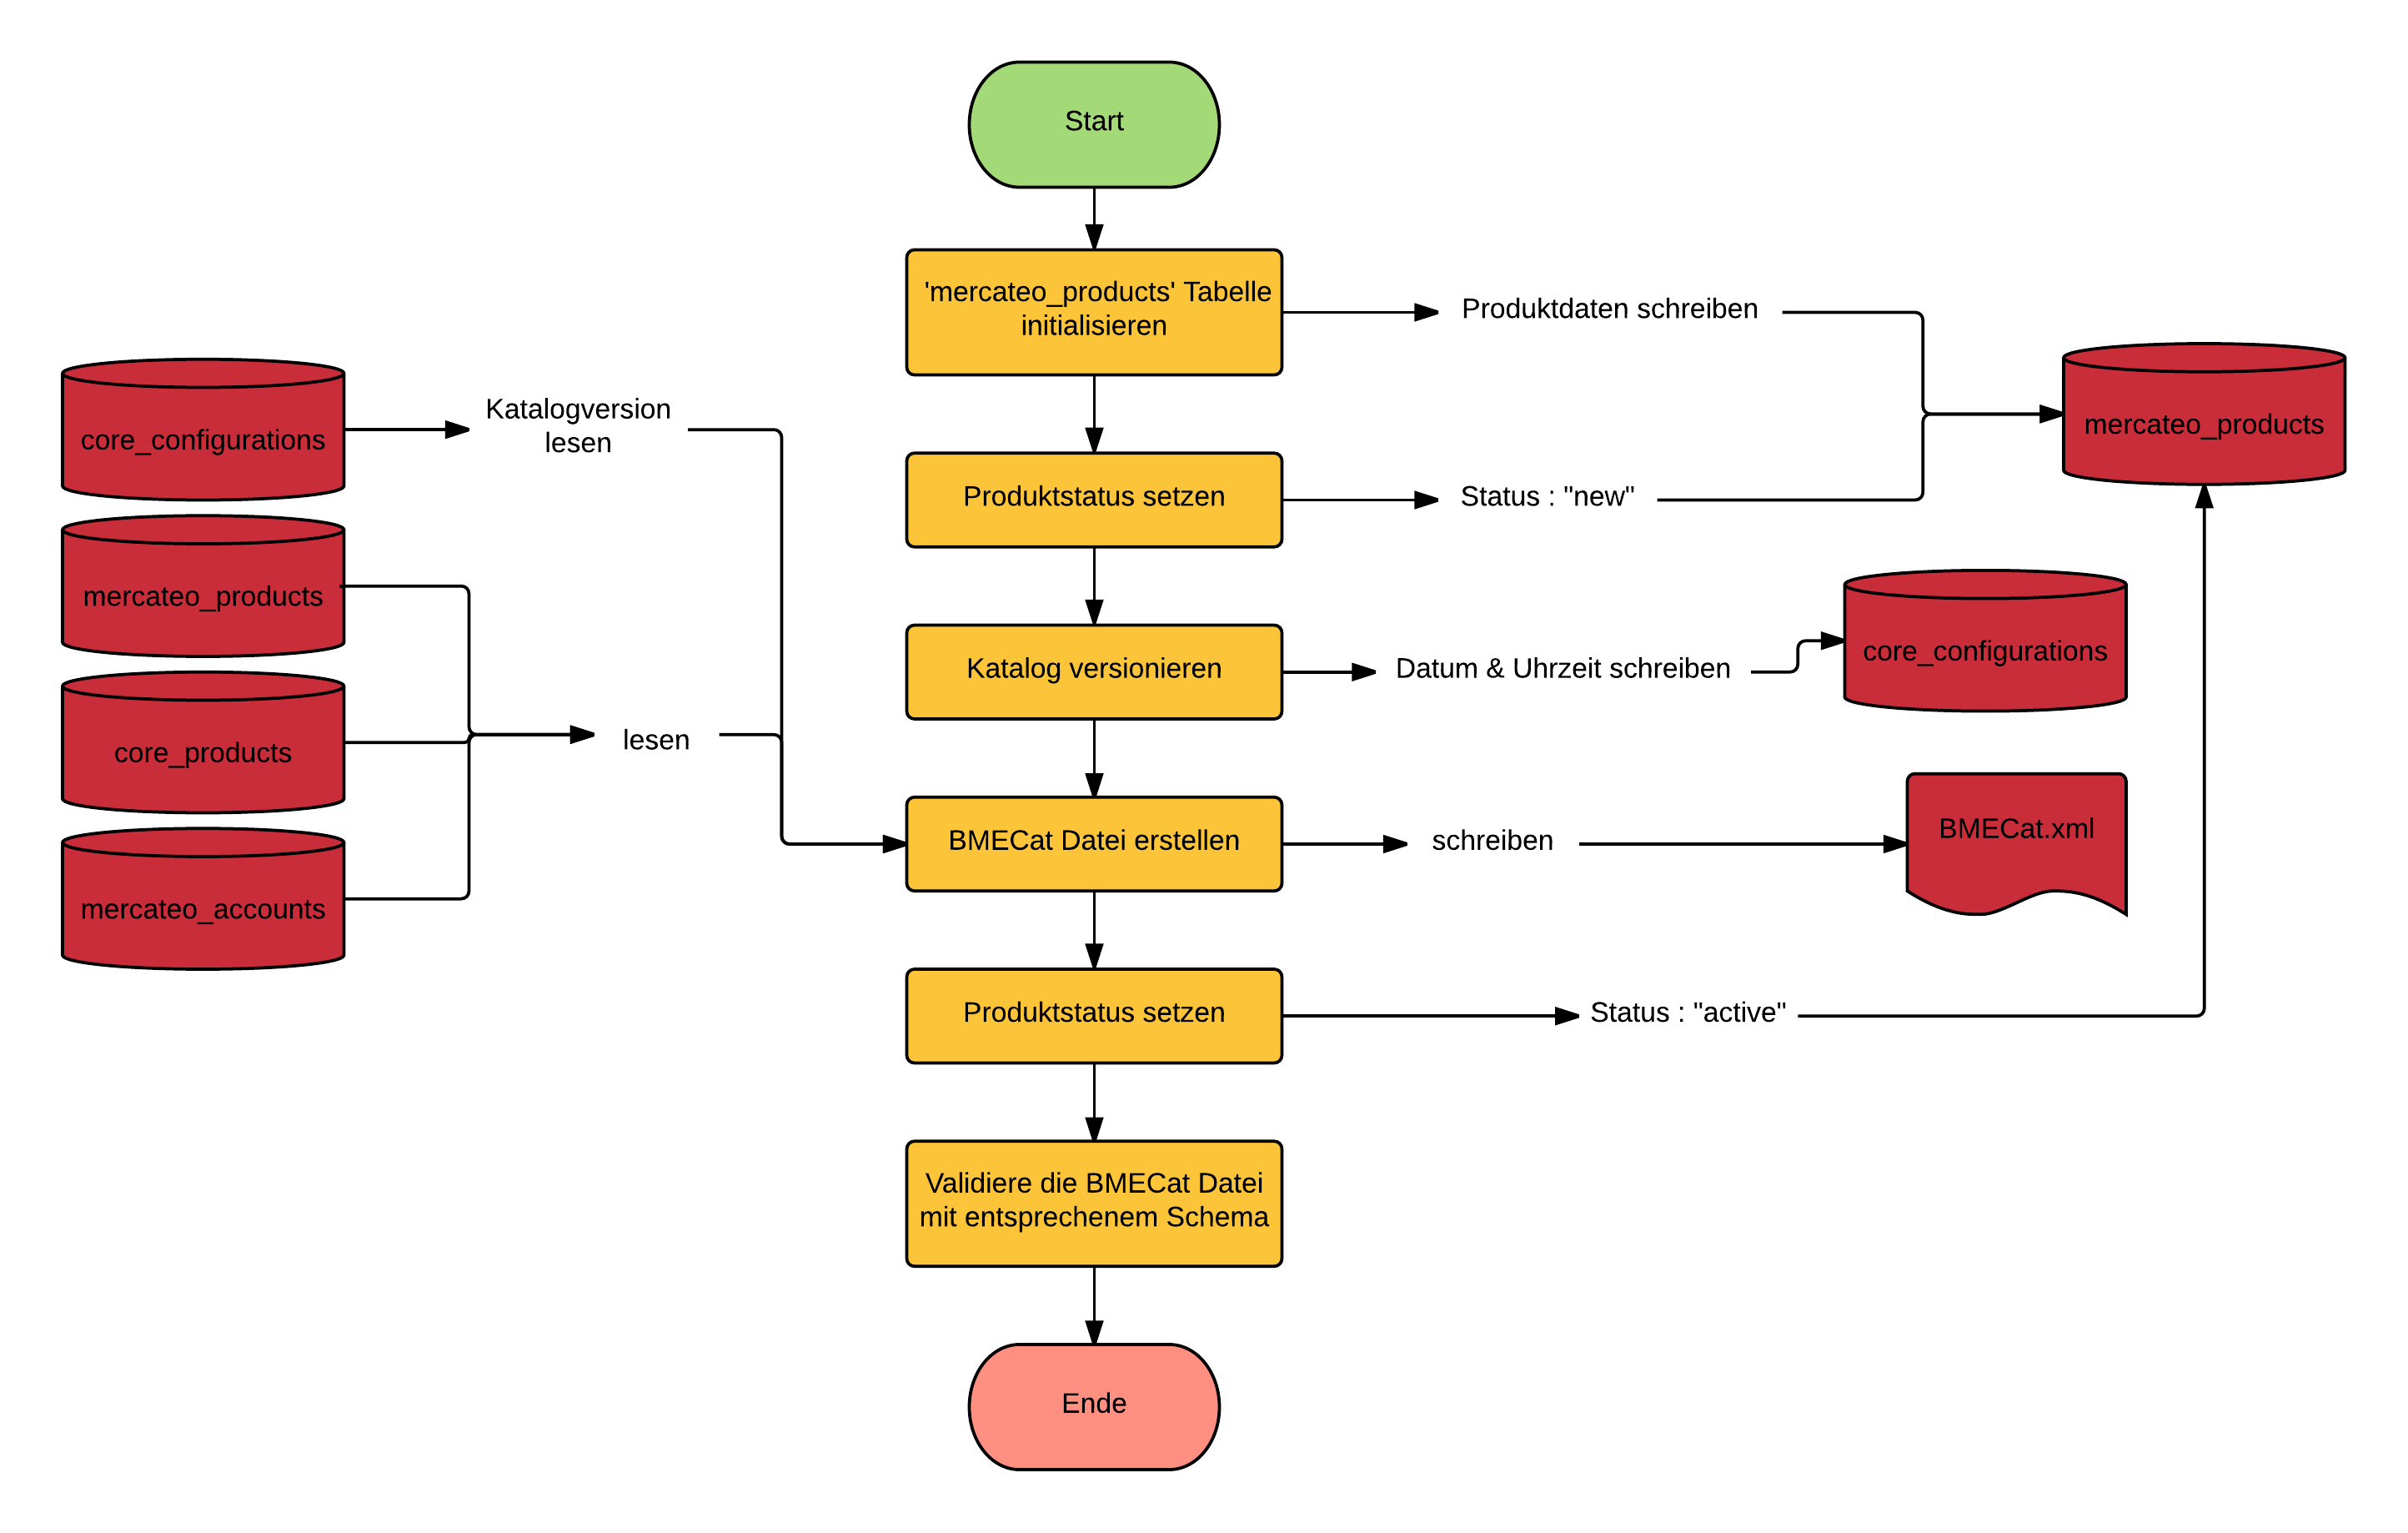
\includegraphics[width=1 \linewidth]{img/newCatalogComplete}
		\captionof{figure}[BasicLogic]{Programmlogik  bei der Transaktion \texttt{T\_NEW\_CATALOG}}
		\vspace{1em}
	\end{minipage}\\
	
	Nachdem das Katalogdokument geschrieben wurde wird es mithilfe des  XSD-Schemas (\texttt{bmecat\_new\_catalog\_1\_2.xsd}) überprüft. 

	\subsubsection{Katalogerstellungslogik in der Klasse \texttt{UpdateCatalogTask} }
    Die	Klasse \texttt{UpdateCatalogTask} realisiert die Umsetzung der Transaktionsart
	\texttt{T\_UPDATE\_PRODUCTS}.
	Bei jedem  Aufruf des Tasks wird zunächst - unter Zuhilfenahme der \texttt{mercateo\_products}-Tabelle - überprüft ob Einträge in der \texttt{core\_products} Tabelle gelöscht, neu hinzugefügt oder geändert wurden. Letzteres geschieht mit Hilfe der Tabelle \texttt{core\_product\_updates} in der jede Änderung an einem \texttt{core\_product} mit dem Zeitstempel der Änderung erfasst wird. Ist einer der Fälle eingetreten wird der Status des Eintrages in der \texttt{mercateo\_products} Tabelle entsprechend gesetzt. \\
	\begin{minipage}{\linewidth}
		\vspace{1em}
		\centering
		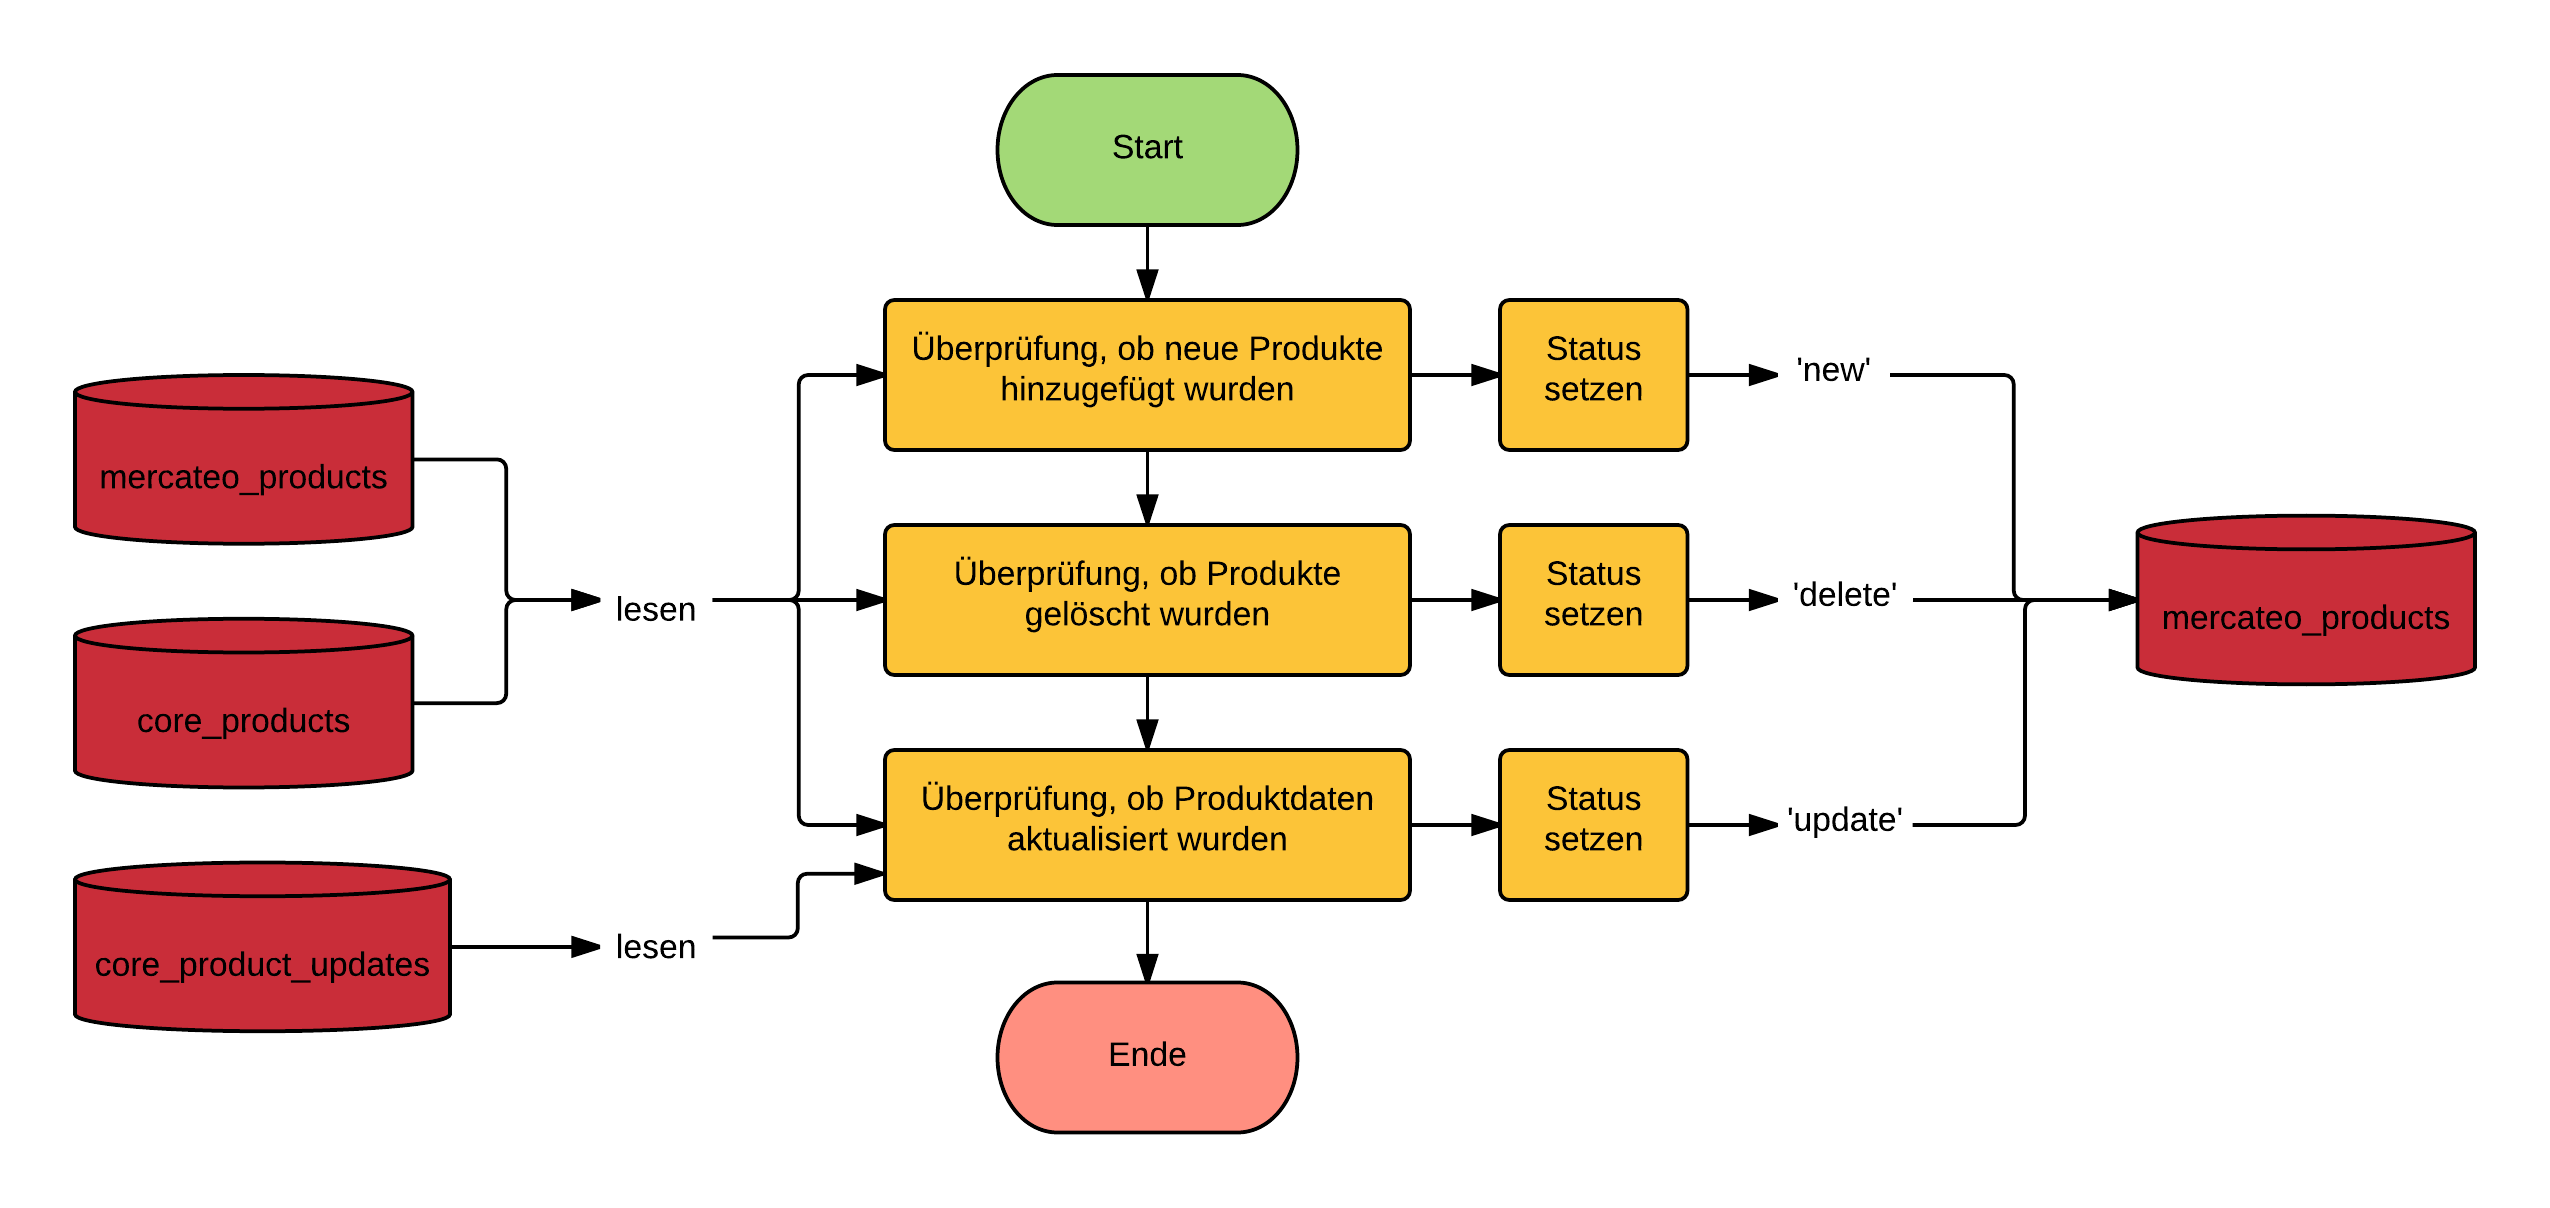
\includegraphics[width=1 \linewidth]{img/productChangeCheck}
		\captionof{figure}[BasicLogic]{Überprüfung auf Produktbestandsänderungen}
		\vspace{1em}
	\end{minipage}\\
	
	
	Anschließend werden wiederum Datum \& Uhrzeit der Erstellung des Katalogdokumentes konstituiert.
	Handelt es sich um die erste Version eines Updatekatalogdokumentes wird das Attribut \texttt{prev\_version} des Elementes \texttt{T\_UPDATE\_PRODUCTS} mit dem initialen Wert von \enquote{0} in die \texttt{core\_configurations} Tabelle geschrieben, um beim darauffolgenden Erstellen der BMECat-Datei direkt wieder ausgelesen und an entsprechender Stelle in das Dokument geschrieben werden zu können.
	Jene Einträge in \texttt{mercateo\_products}, die den Status \texttt{delete} haben, werden gelöscht, danach wird der Status der Übrigen auf \texttt{active} gesetzt und  der Wert des Attributes \texttt{prev\_version} um \enquote{1} erhöht. Abschließend erfolgt die Validierung des Dokumentes mithilfe des Schemas \texttt{bmecat\_update\_products\_1\_2.xsd}.
	
	\begin{minipage}{\linewidth}
		\vspace{1em}
		\centering
		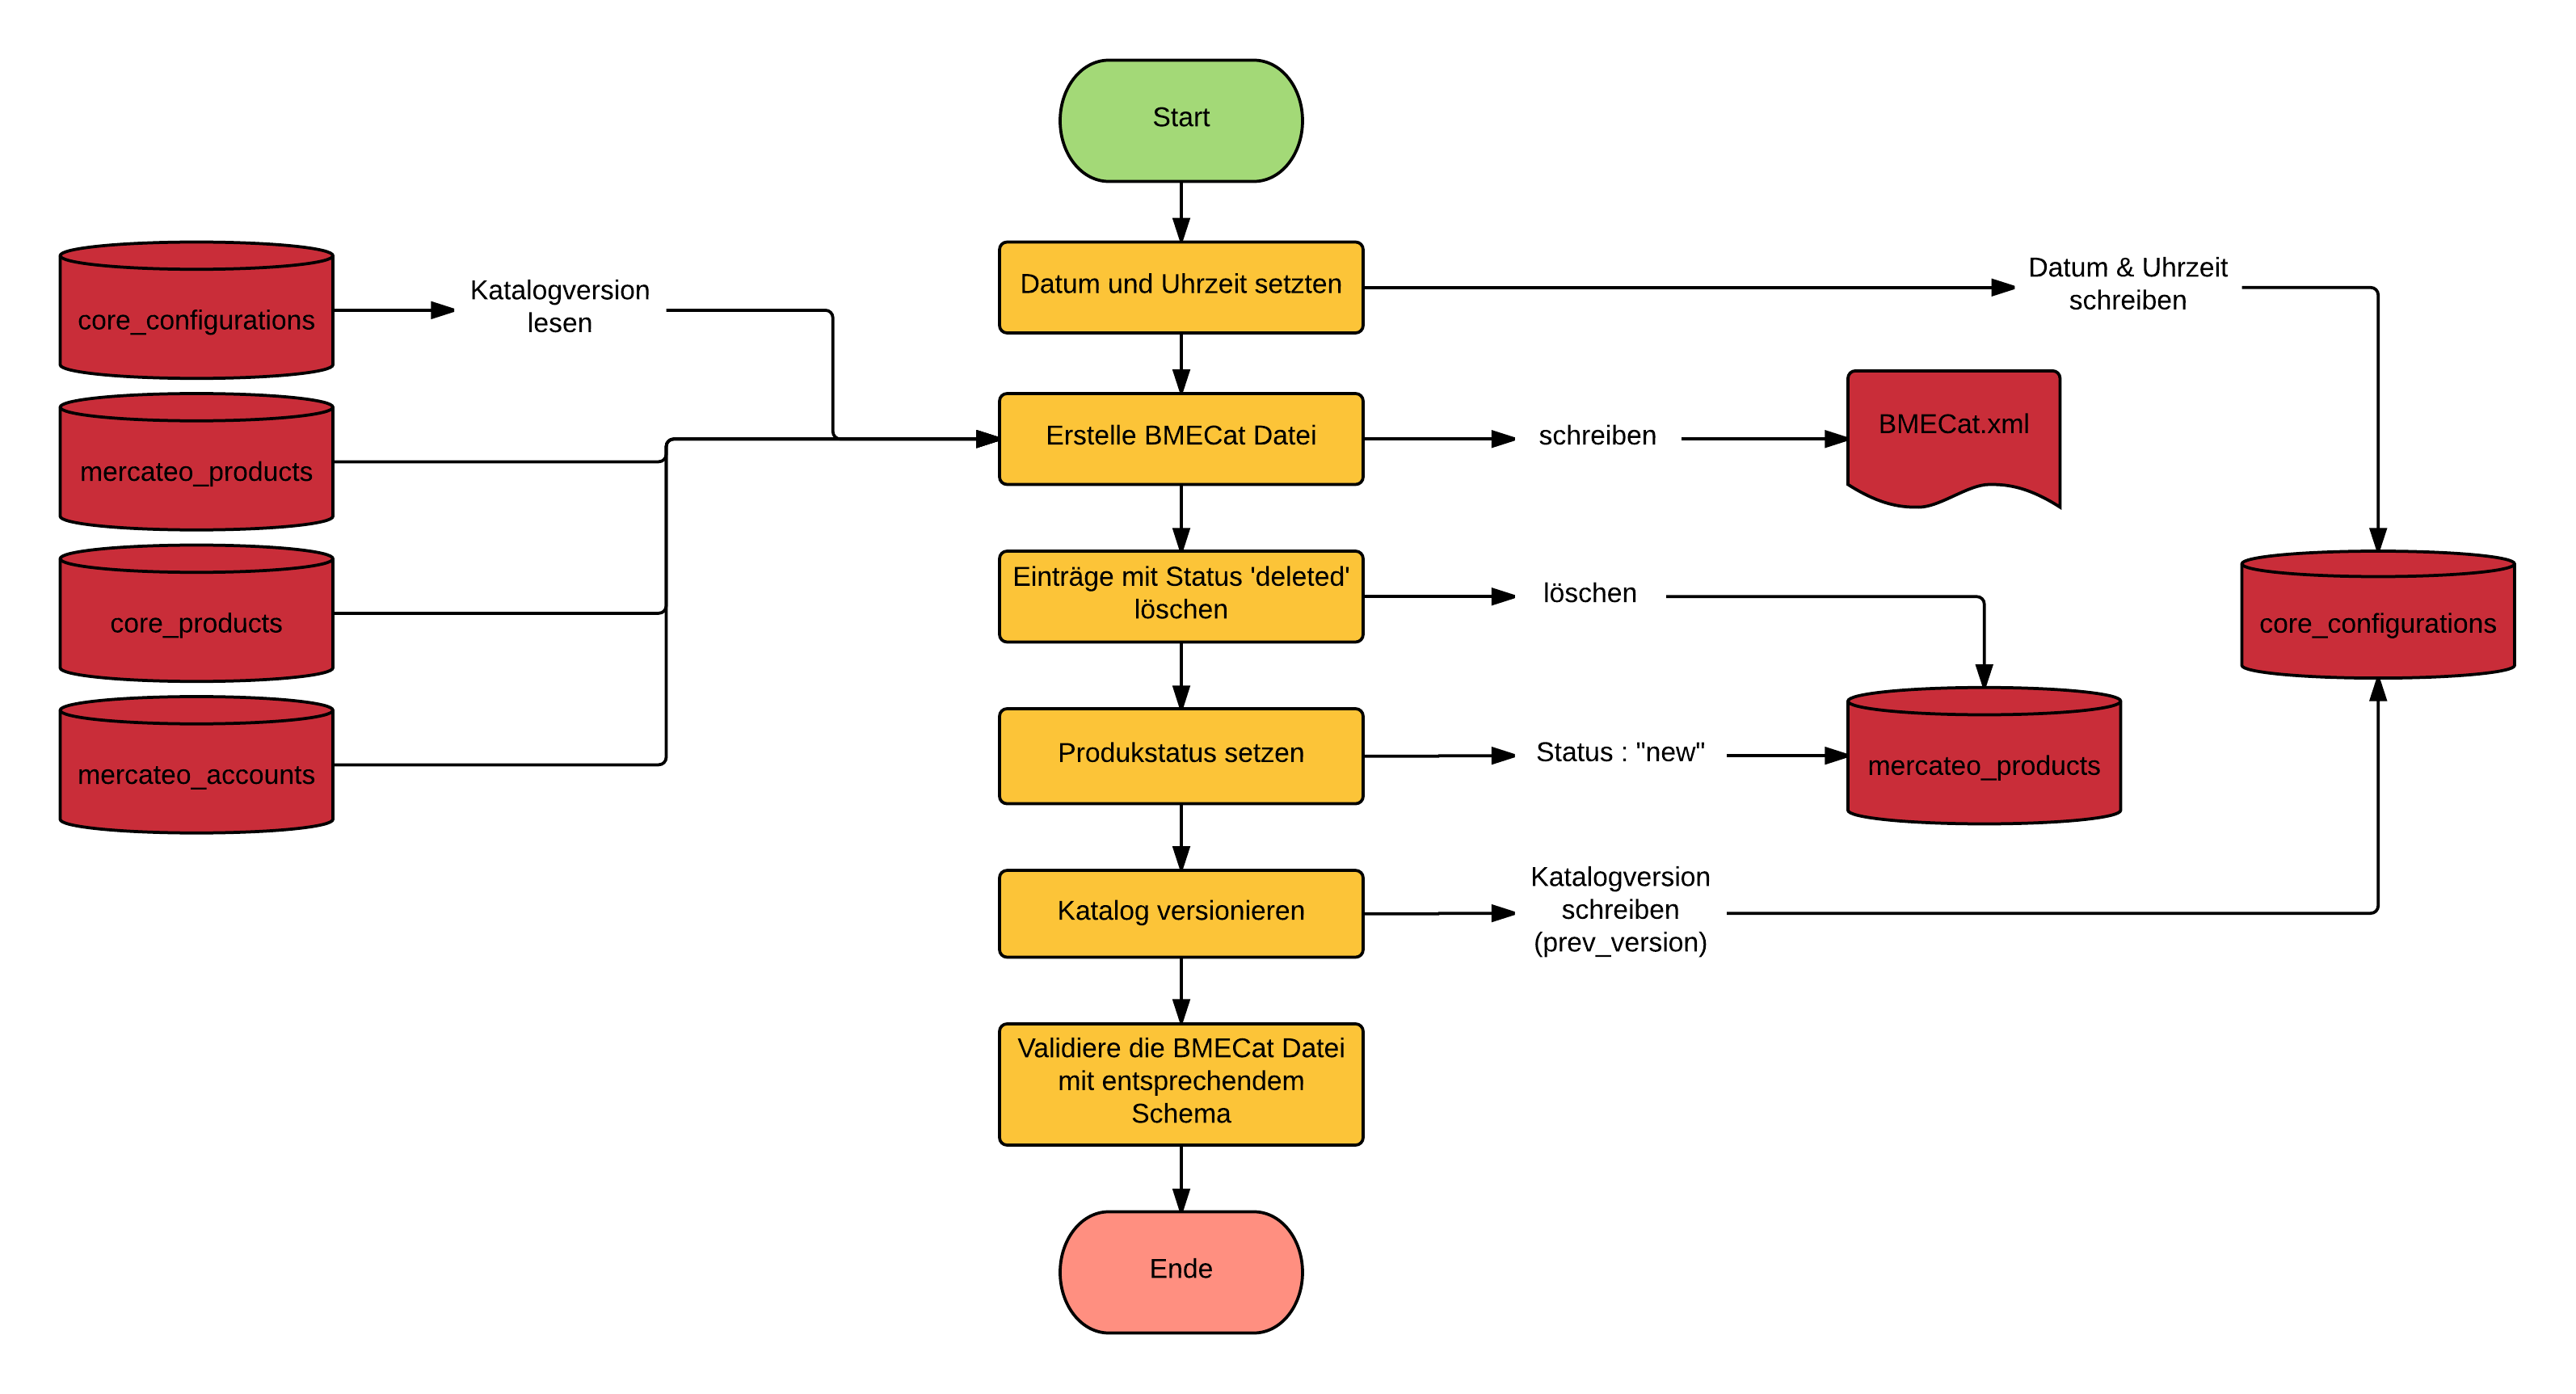
\includegraphics[width=1 \linewidth]{img/updateCatalogComplete}
		\captionof{figure}[BasicLogic]{Programmlogik  bei der Transaktion \texttt{T\_UPDATE\_PRODUCTS}}
		\vspace{1em}
	\end{minipage}\\
	
	\
	
	\subsection{Bestandsdatenabfrage}
	
	Mercateo 
	Die Bestandsdatenabfrage wird mit einem Controller realisiert, dessen \texttt{index()} Funktion als Parameter die angefragte SKU hat.
	Von Seiten Mercateos kann so eine URL der Form \url{http://itool.local/mercateo/availability/12} aufgerufen werden. Ist die SKU im System vorhanden, wird die Bestandsmenge als Integer Wert zurückgeliefert, ist die angefragte SKU nicht im System, wird eine Fehlermeldung ausgegeben.
	
	\section{Implementierung}
	
	Die Implementierung gliedert sich demnach in 2 Bereiche, die Konsolenanwendung zur Generierung des Katalogdokumentes und die Bestandsdatenabfrage.
	
	\subsection{Die PrepareCatalog Shell}
	
	Mit der PrepareCatalog Shell wird der Entwurf zur Erzeugung eine BMECat Katalogdokumentes umgesetzt. Die eigentliche Shell Klasse \texttt{PrepareCatalogShell} dient in der Implementierung  dazu die Subcommandos \texttt{AddNewCatalogTask}, \texttt{UpdateCatalogTask} und \texttt{DeleteCatalogTask} aufzurufen und sicherzustellen, dass die notwendigen Argumente übergeben werden.
	\lstset{basicstyle=\scriptsize\ttfamily}
	\begin{lstlisting}
	Usage:
	cake mercateo.prepare_catalog [subcommand] [-h] [-q] [-v] <Core Seller Id>
	
	Subcommands:
	
	addNewCatalog  Creates a new BMECat Catalog file.
	deleteCatalog  Deletes Sellers Products from mercateo_products table
	updateCatalog  Creates an Update Catalog file.
	
	To see help on a subcommand use `cake mercateo.prepare_catalog [subcommand] --help`
	
	Options:
	
	--help, -h     Display this help.
	--quiet, -q    Enable quiet output.
	--verbose, -v  Enable verbose output.
	
	Arguments:
	
	Core Seller Id  The ID of the Seller for whom the BMECat shall be
	            created

	
	\end{lstlisting}
	
	Kann der übergebene Parameter keinem Verkäufer zugeordnet werden wird eine Übersicht der verfügbaren Verkäufer angezeigt. Dies geschieht in den einzelnen Tasks über die geerbte Methode \texttt{validateArgument(\$coreSellerId)}.
	
	\begin{lstlisting}
	Please choose one of the available Sellers:
	
	ID | Name
	
	1  | Hendrik
	2  | Ben
	3  | Guehring
	\end{lstlisting}
	
	Dabei liegt dem Programm folgende Aufrufhierarchie zugrunde:\\
	\begin{minipage}{\linewidth}
		\vspace{1em}
		\centering
		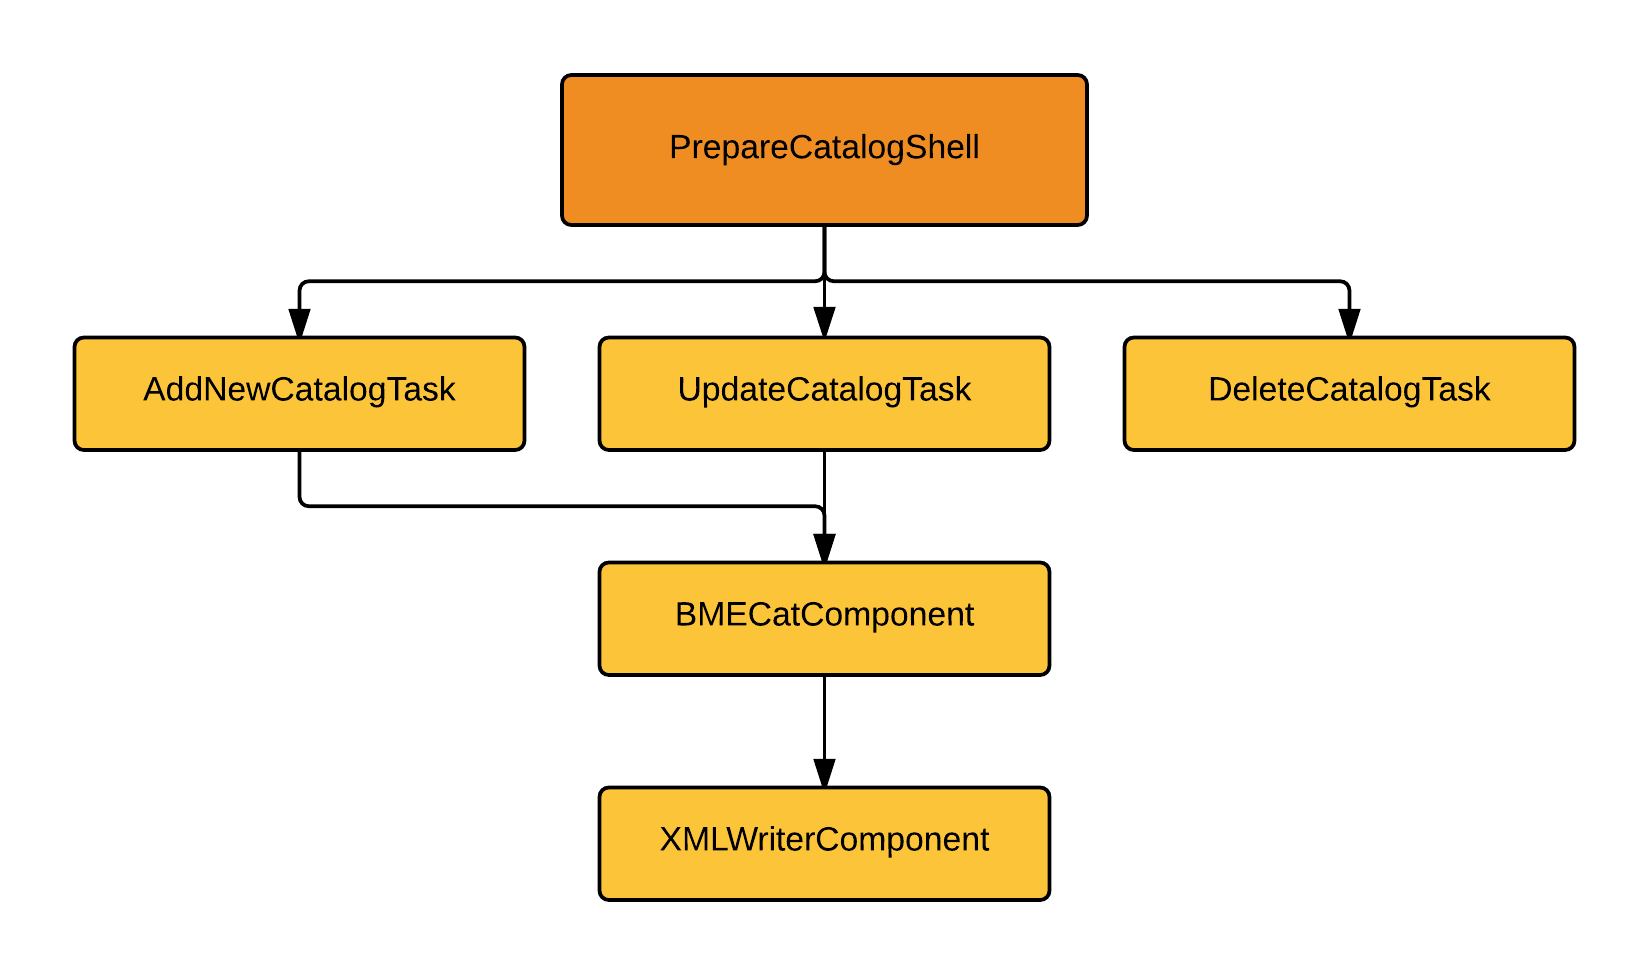
\includegraphics[width=0.7 \linewidth]{img/Aufrufhierarchie}
		\captionof{figure}[BasicLogic]{Aufrufhierarchie PrepareCatalogShell}
		\vspace{1em}
	\end{minipage}\\
	
	
	
	
	Im Folgenden werden die einzelnen Klassen vorgestellt.
	
	\subsection{XMLWriterComponent}
	
	Die XMLWriterComponent Klasse ist insofern wichtiger Bestandteil der Implementierung, als das ohne sie nur auf umständlicherem Wege XML geschrieben werden kann. Hier seien nun in Kürze jene Methoden vorgestellt, die von der Klasse BMECatComponent genutzt werden:
	
	\begin{enumerate}[noitemsep]
	\item \texttt{public function openXmlWriter(\$filePath, \$rootElement, \$attributes = null, \$doctype = null)} \\
		  Ermöglicht das Anlegen einer neuen XML Datei mit der Option Attribute ( z.B. die BMECat-Version) zu übergeben, sowie über den DOCTYPE eine entsprechende .dtd Datei zu referenzieren.
	\item \texttt{public function closeXmlWriter()} \\
		  Schließt das XML Dokument ab.
	\item \texttt{writeXmlElement(\$name, \$value, \$type = "text", \$attributes = [])}\\
		  Schreibt ein XML Element mit dem übergebenen Wert und den dazugehörigen Attributen und schließt es sogleich ab. (Schreibt Start- und End Tag)
	\item \texttt{public function writeStartXmlElement(\$name, \$attributes = [])}\\
		  Öffnet ein XML Element und setzt die übergebenen Attribute. (Schreibt den Start-Tag)
	\item \texttt{public function writeEndXmlElement()}\\
		  Schließt das zuvor geöffnete Element ab. (Schreibt den End-Tag)
	\end{enumerate}
	
	VORTEILE? 
	
	\subsection{BMECatComponent}
	
	Die Klasse BMECatComponent dient dazu ein wohlgeformtes und gültiges XML Dokument entsprechend den BMECat- und Mercateo Vorgaben zu erstellen. \\
	\begin{minipage}{\linewidth}
		\vspace{1em}
		\centering
		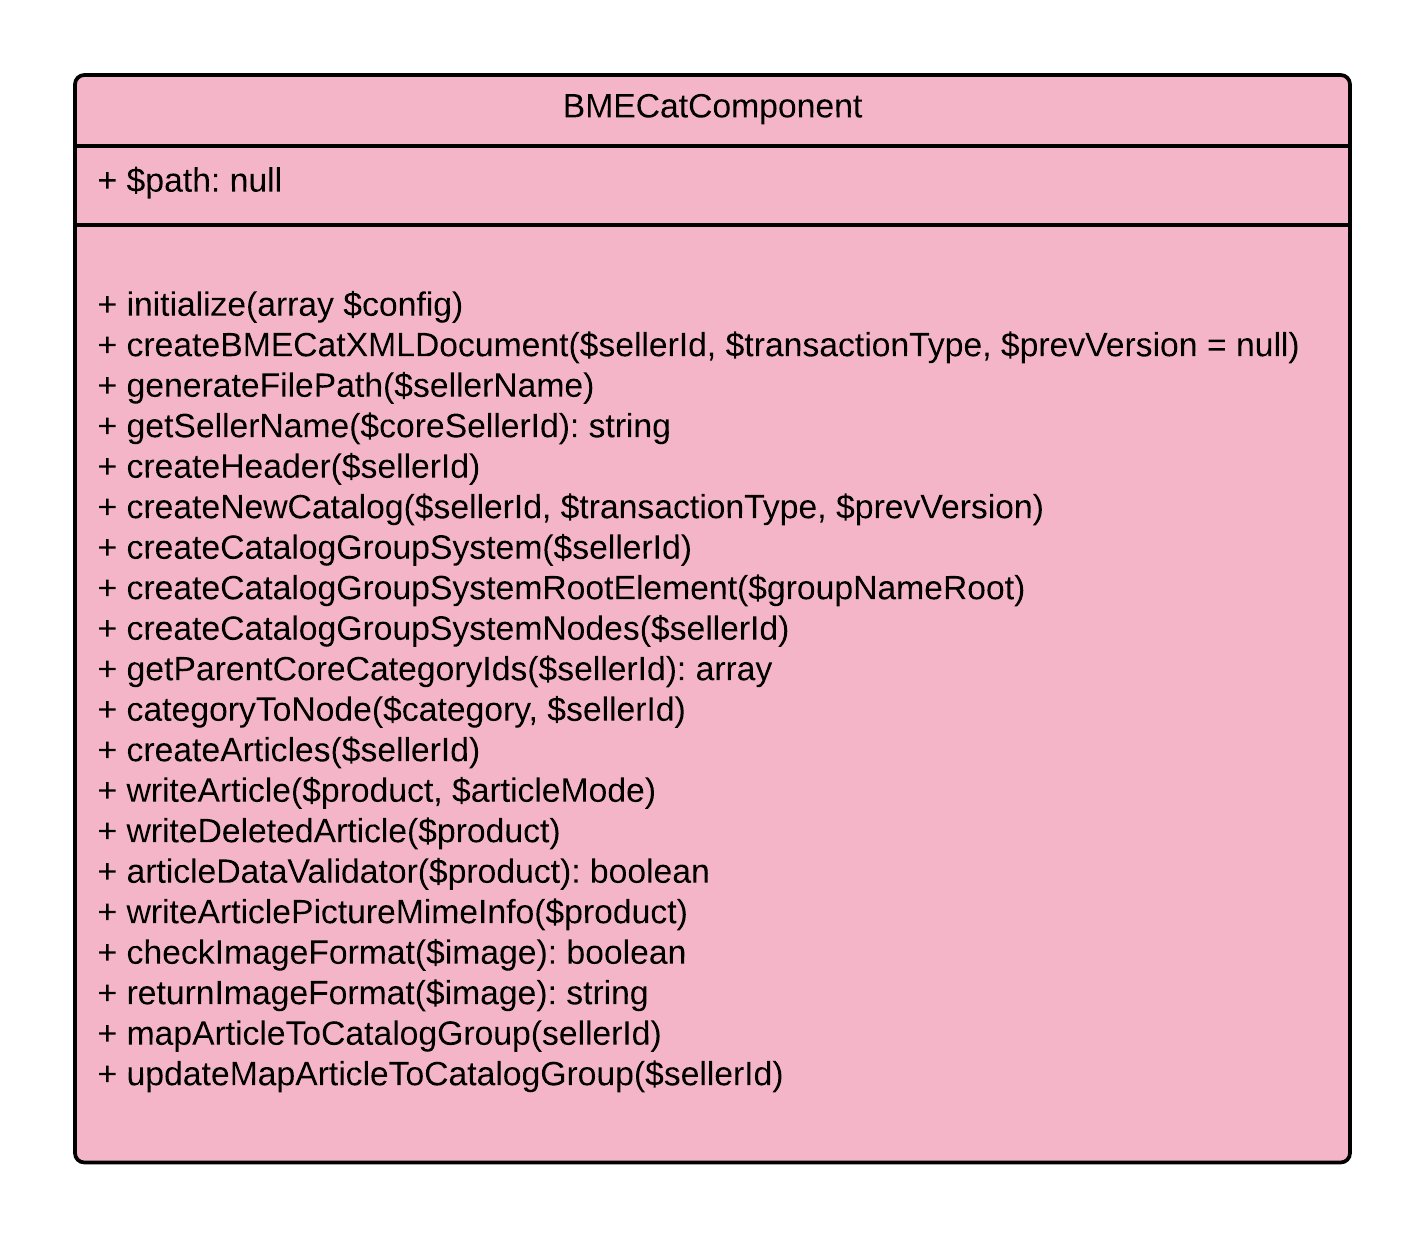
\includegraphics[width=0.8 \linewidth]{img/BMECatComponentUML}
		\captionof{figure}[BasicLogic]{UML Diagramm der Klasse BMECatComponent}
		\vspace{1em}
	\end{minipage}
	Wie im Kapitel Grundlagen bereits beschrieben gliedert sich ein BMECat Dokument in 4 Bereiche und zwar den Header, das Kataloggruppensystem, die Auflistung der einzelnen Artikel und die Zuordnung der Artikel zu ihren Kategorien. Der BMECat Komponent stellt für jeden dieser Teilbereiche Funktionen bereit die in Folge erläutert werden sollen.
	Zur Orientierung dient eine Übersicht der Aufrufhierarchie.\\
	
	\begin{minipage}{\linewidth}
		\vspace{1em}
		\centering
		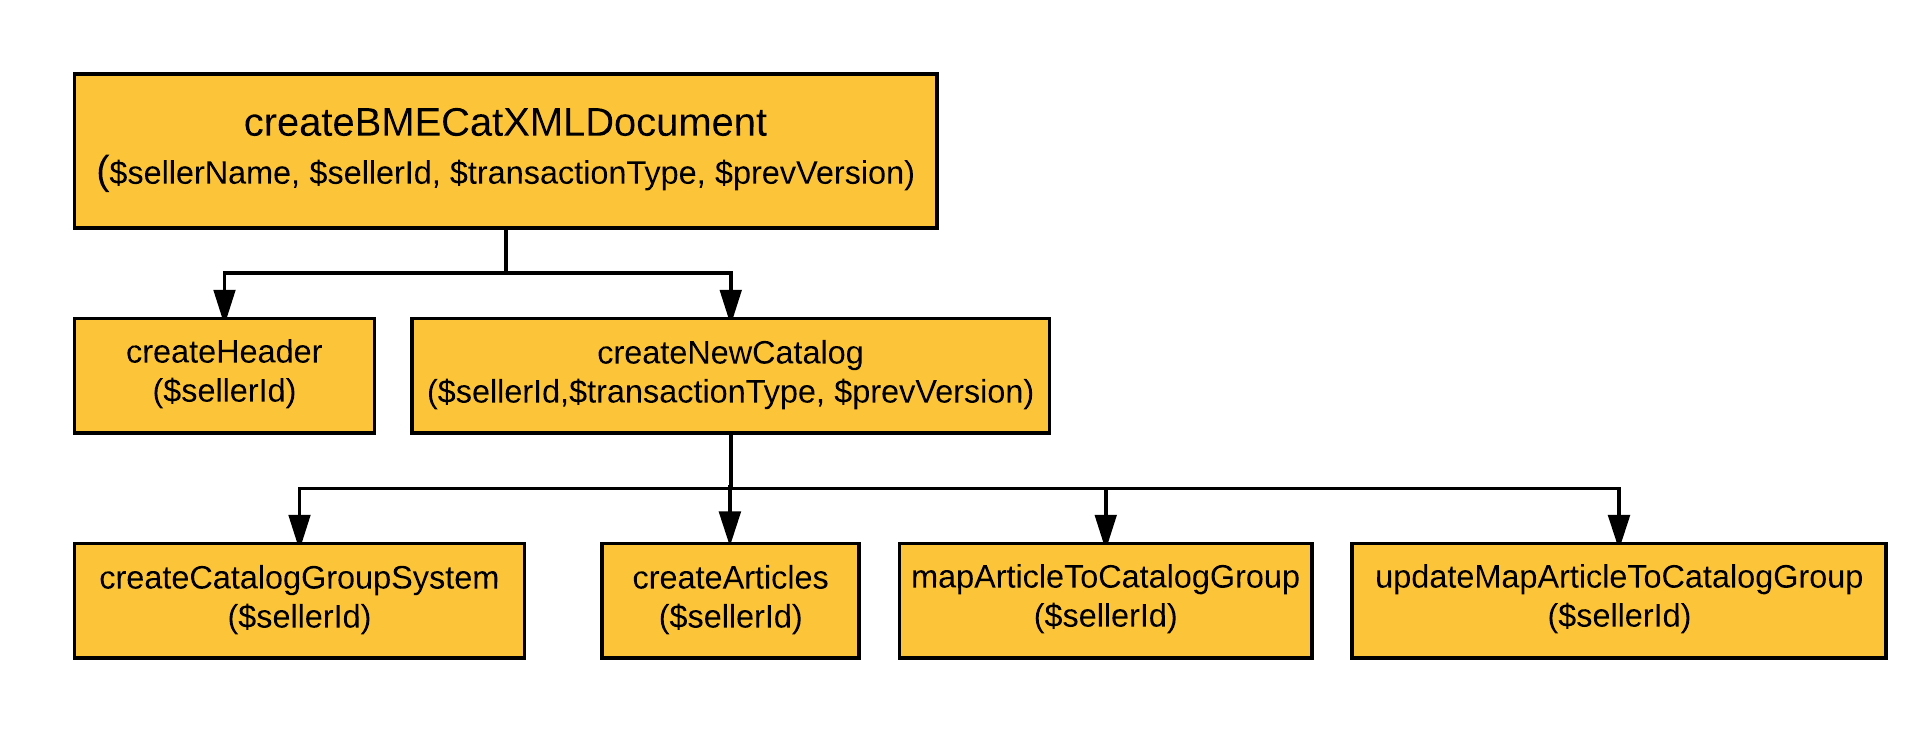
\includegraphics[width=0.8 \linewidth]{img/createBMECatHierarchie}
		\captionof{figure}[BasicLogic]{Aufrufhierarchie createBMECatXMLDocument}
		\vspace{1em}
	\end{minipage}
	
	
	
	
	
	\subsubsection{Erstellen des BMECat Dokumentes}
	
	Die Funktion \texttt{createBMECatXMLDocument(\$sellerName, \$sellerId, \$transactionType, \$prevVersion)} dient der Erzeugung eines BMECat Dokumentes. Sie legt die XML Datei mit der Namenskonvention \texttt{\enquote{Verkäufername\_Erzeugungsdatum\_Erzeugungszeit.xml}} an und schreibt Informationen zum XML Namensraum \textit{(xmlns)} und zur Dokumenttypdefinition \textit{(dtd)} in die XML-Deklaration. Von ihr werden die Methoden zur Erzeugung des Headers und der restlichen Abschnitte des BMECat Dokumentes aufgerufen.
	Anhand des Parameters \texttt{\$transactionType} wird entschieden ob bei dem zu erzeugenden Dokument die Transaktion \texttt{T\_NEW\_CATALOG} oder \texttt{T\_UPDATE\_PRODUCTS} umgesetzt werden soll. Falls die Datei, z.B. wegen fehlender Rechte, nicht angelegt werden kann, wird durch die XMLWriter Komponente eine Exception erzeugt.
	
	\subsubsection{Schreiben der Header Sektion}

	Die Methode \texttt{createHeader(\$sellerId)} schreibt die BMECat-Header-Sektion des Dokumentes. Alle benötigten Informationen, wie z.B. Herstellername oder Katalogversion werden dabei anhand der \texttt{sellerId} aus der \texttt{mercate\_accounts} Tabelle geladen.
	
	\subsubsection{Schreiben des Kataloggruppensystems}
	
	Die Methode \texttt{createCatalogGroupSystem(\$sellerId)} steuert die Erzeugung des Kataloggruppensystems. Die von ihr aufgerufenen Methoden sind im wesentlichen für das Schreiben bestimmter XML Elemente zuständig.\\
	\begin{minipage}{\linewidth}
		\vspace{1em}
		\centering
		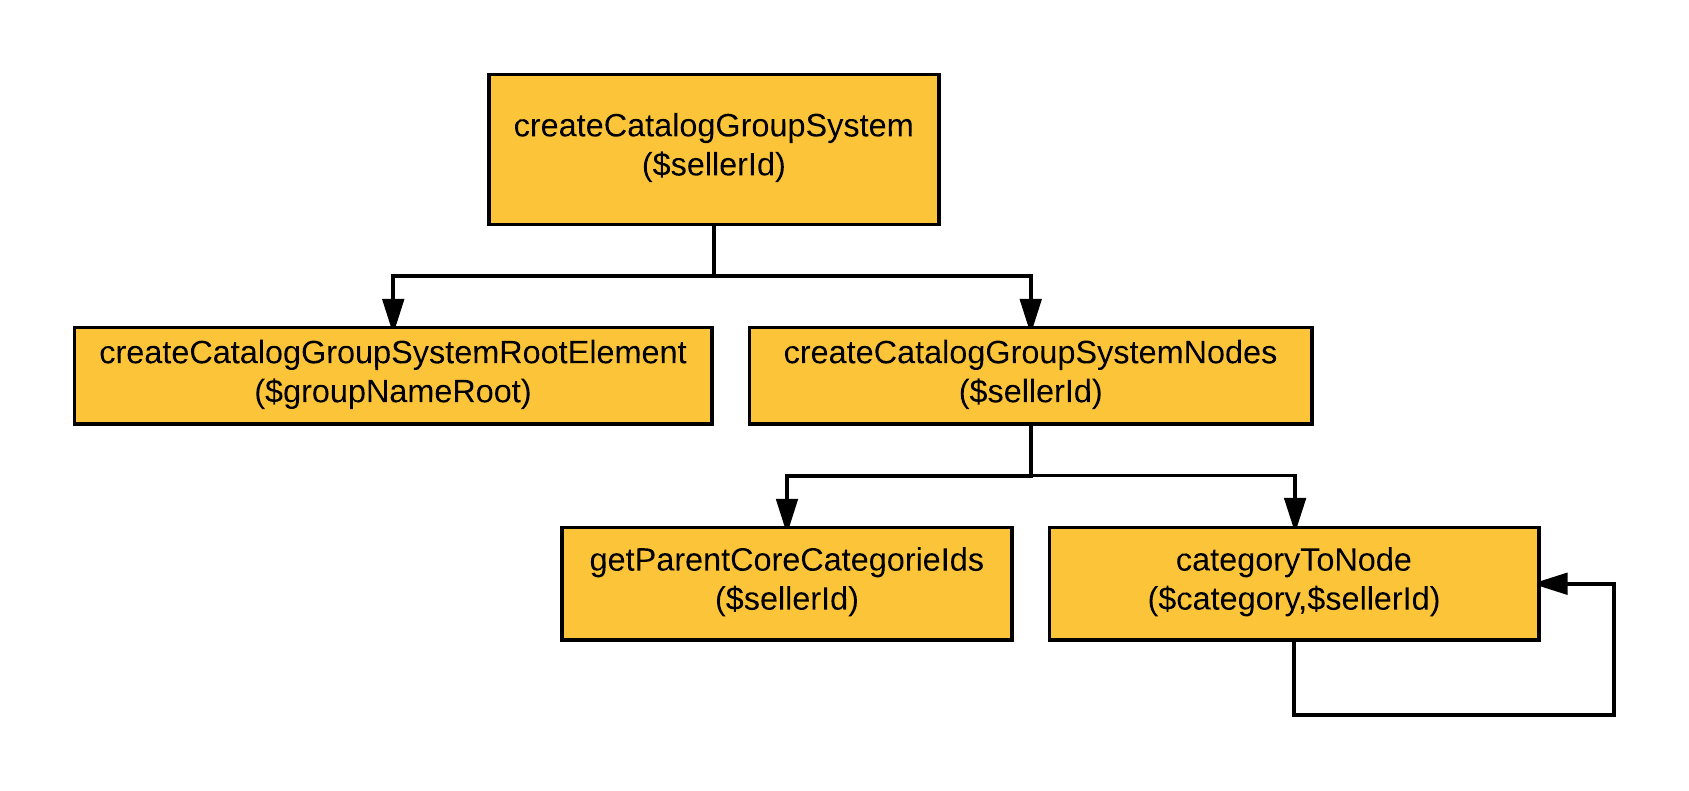
\includegraphics[width=0.7 \linewidth]{img/CreateCatalogGroupSystemHierarchie}
		\captionof{figure}[BasicLogic]{Aufrufhierarchie createCatalogGroupSystem}
		\vspace{1em}
	\end{minipage}
	
	 Das tatsächliche Abbilden der Katalogstruktur erfolgt in der Methode \texttt{categoryToNode(\ \$category,\$sellerId)}.
	 
	\begin{addmargin}[1cm]{1cm}
	\underline{Dazu ein kleiner Exkurs:}\\
		 CakePHP bietet die Möglichkeit einem Model ein sogenanntes Tree-Behaviour hinzuzufügen. Dieses basiert auf dem Nested-Set-Konzept, das es ermöglicht hierarchische Strukturen in relationalen Datenbanken abzubilden\footnote{vgl. hierzu: \url{https://www.sitepoint.com/hierarchical-data-database-2/}}. Die \texttt{core\_categories} Tabelle bedient sich dieses \enquote{Behavious}, was es ermöglicht diesen Kategoriebaum rekursiv zu durchlaufen und dadurch das Kataloggruppensystem des BMECat abzubilden.
	\end{addmargin}
	
	
	Die Methode \texttt{categoryToNode(\$category,\$sellerId)} durchläuft, ausgehend vom Wurzelelement, alle Kindelemente und schreibt die entsprechenden Daten in das Dokument. Solange dabei die Anzahl der Kindelemente des gerade traversierten Elementes größer 0 ist wird dabei dem Attribut \texttt{type} der Wert \texttt{node} zugewiesen. Gibt es keine Kindelemente mehr, wird der Wert auf \texttt{leaf} gesetzt. 
	\lstset{language=xml}
	\begin{lstlisting}
	<CATALOG_STRUCTURE type="node">
	 <GROUP_ID>207</GROUP_ID>
	 <GROUP_NAME>Auto -Motorrad - Flugzeug</GROUP_NAME>
	 <PARENT_ID>202</PARENT_ID>
	</CATALOG_STRUCTURE>
	<CATALOG_STRUCTURE type="leaf">
	 <GROUP_ID>210</GROUP_ID>
	 <GROUP_NAME>Oldtimer</GROUP_NAME>
	 <PARENT_ID>207</PARENT_ID>
	</CATALOG_STRUCTURE>
	\end{lstlisting}
	
	\subsubsection{Artikelerstellung}
	
	Die Methode \texttt{createArticles(\$sellerId)} aggregiert die zu schreibenenden Artikeldaten. Über einen \texttt{INNER JOIN} werden die Tabellen \texttt{mercateo\_products} und \texttt{core\_products} verbunden, so dass über die in \texttt{mercateo\_products} hinterlegte \texttt{core\_product\_id} die entsprechenden Daten aus der \texttt{core\_products} Tabelle nachgeladen werden können. 
	Ist der Artikelstatus gleich \textit{\enquote{new}} oder \textit{\enquote{update}} wird die Methode \texttt{writeArticle(\$product, \$articleMode)} aufgerufen, die die entsprechenden XML Elemente schreibt. \\
		
		\begin{minipage}{\linewidth}
			\vspace{1em}
			\centering
			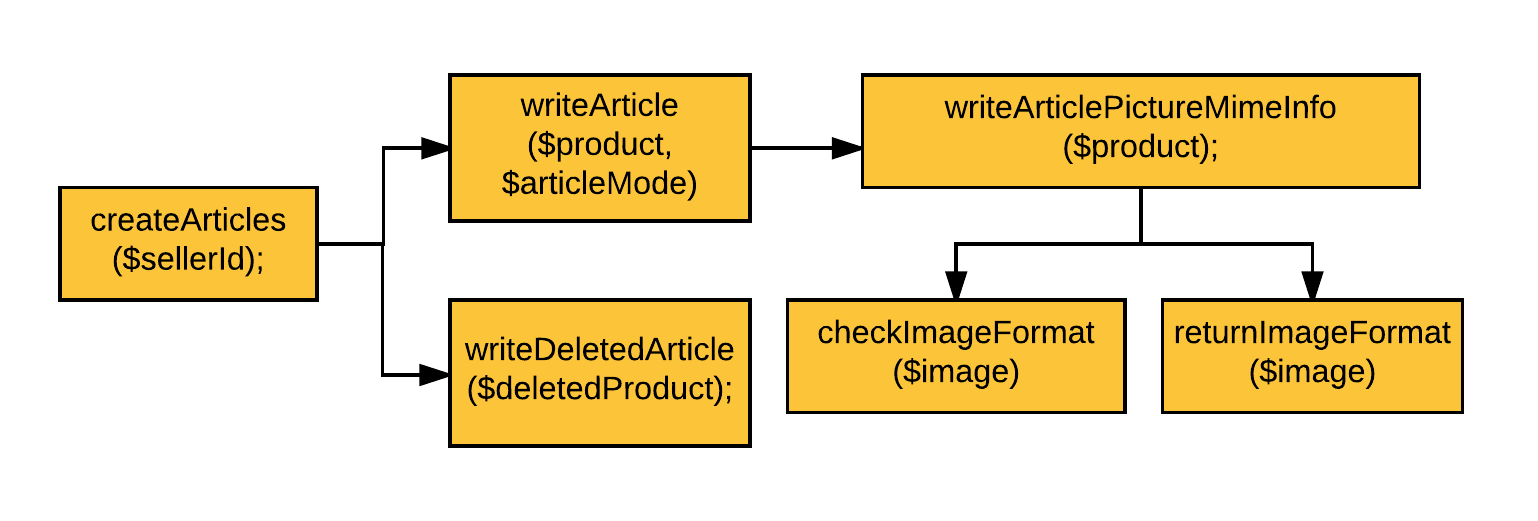
\includegraphics[width=0.7 \linewidth]{img/createArticleHierarchie}
			\captionof{figure}[BasicLogic]{Aufrufhierarchie createArticle}
			\vspace{1em}
		\end{minipage}
	
	Zusätzlich wird geprüft ob die dem Artikel zugeordneten Bilder der Mercateo Spezifikation entsprechen. Diese gestattet als Bildformate nur \enquote{.jpeg} und \enquote{.gif}. Entsprechen die Bilddateien nicht diesem Format wird eine entsprechende Ausnahmebehandlung durchgeführt. Dabei wird der komplette Pfad der beanstandeten Datei zurückgeliefert, um es dem Anwender zu erleichtern diesen Fehler zu beheben.\\
	
	\begin{lstlisting}
	2017-01-05 16:30:55 Info: Product with CoreProductId: 7147 updated
	Exception: 'png' ist not allowed as File Extension.
	Only .gif & .jpg Files are accepted by Mercateo-Marketplace
	Check Image Path: https://bild-im-rahmen.com/wp-content/uploads/2016/03/s21r.png
	\end{lstlisting}

	Handelt es sich um einen gelöschten Artikel, wird die Methode \texttt{writeDeletedArticle(\$pro\-duct)} aufgerufen. Diese schreibt die in \texttt{mercateo\_products} hinterlegten, um einen Artikel als gelöscht auszeichnen zu können notwendigen Informationen - Die SKU \& den Titel sowie den Wert des Artikelattributes \texttt{mode} (hier \texttt{delete})- in das Dokument.
	
	\subsubsection{Kategoriemapping}
	
	Mit der Methode \texttt{mapArticleToCatalogGroup(\$sellerId)} werden bei der Transaktion \texttt{T\_NEW\_CATALOG} die Artikel ihren Kategorien zugewiesen. Alle dazu notwendigen Informationen finden sich in der \texttt{mercateo\_products} Tabelle.
	
	Wird ein Update Katalog erstellt wird die Funktion \texttt{updateMapArticleToCatalogGroup(\$sellerId)} aufgerufen. Sie setzt den bei der Transaktion \texttt{T\_UPDATE\_PRODCUTS} geforderten Attributwert für \texttt{mode} entsprechend der Angaben in der \texttt{mercateo\_products} Tabelle.
	Mögliche Werte sind \textit{\enquote{new}} für neu erstellte und \textit{\enquote{delete}} für gelöschte Produkte.
	
	\subsection{Die Klasse \texttt{CatalogToolsTask}}
	
	Die Klasse \texttt{CatalogToolsTask} stellt Methoden zur Verfügung die von den drei sie beerbenden Task Klassen verwendet werden.
	
	\begin{minipage}{\linewidth}
		\vspace{1em}
		\centering
		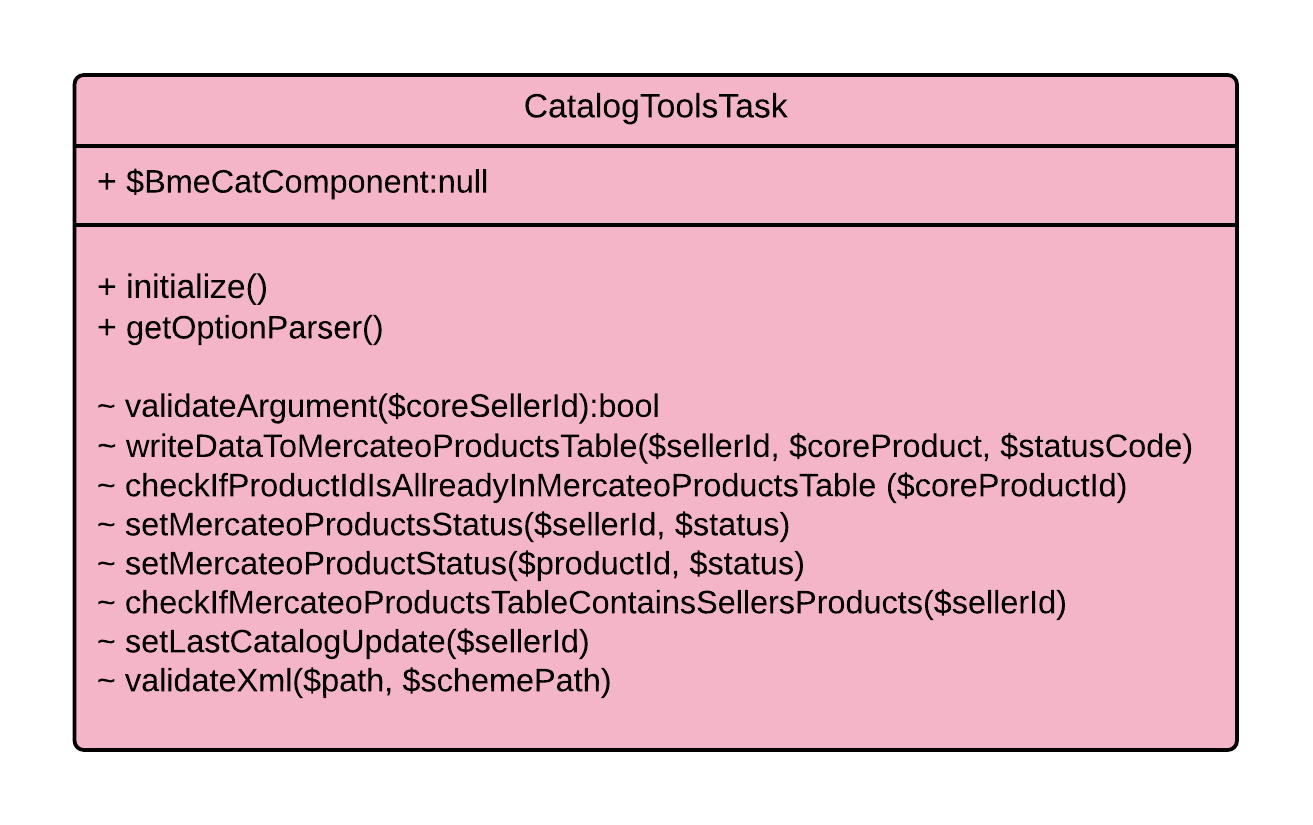
\includegraphics[width=0.7 \linewidth]{img/CatalogToolsTaskUML}
		\captionof{figure}[BasicLogic]{UML Diagramm der Klasse CatalogToolsTask}
		\vspace{1em}
	\end{minipage}
	
	Die Methode \texttt{initialize()} lädt alle zur Katalogerzeugung benötigten Model-Klassen und initialisiert die Instanzvariable \texttt{BMECatComponent}.
	Die vom CakePHP-Framework zur Verfügung gestellte Methode \texttt{getOptionParser()} überprüft, ob beim Aufruf des Tasks die benötigte \texttt{\$coreSellerId} übergeben wird.
	Mit \texttt{validateArgument(\$coreSellerId)} wird geprüft, ob die übergebene \texttt{\$coreSellerId} im System vorhanden ist. Falls ja, wird \texttt{true} zurückgeliefert. Falls nicht, wird eine tabellarische Übersicht der verfügbaren Verkäufer ausgegeben und \texttt{false} zurückgegeben.
	Durch \texttt{writeDataToMercateoProductsTable(\$sellerId, \$coreProduct, \$statusCode)} werden Einträge in der \texttt{mercateo\_products}-Tabelle erzeugt, dabei wird mit Aufruf der \texttt{MercateoProducts}-Model-Methode \texttt{allreadyInDatabase(\$coreProductId)} sichergestellt, dass keine doppelten Einträge erstellt werden, eine bestimmte \texttt{core\_product\_id} also nur einmal in der Tabelle vorkommt. Das setzten eines bestimmten Produktstatus für \textit{einen} Eintrag in der \texttt{mercateo\_products}-Tabelle wird mit der Methode \texttt{setMercateoProductStatus(\$productId, \$status)} realisiert. Das setzten der Produkstatus aller Produkte eines \textit{CoreSellers} geschieht mit \texttt{setMercateoProductsStatus(\$sellerId, \$status)}.
	 Die Methode \texttt{setLastCatalogUpdate(\$sellerId)} schreibt den Timestamp der letzten Katalogerstellung in die \texttt{core\_configurations}-Tabelle.\\
	
	\begin{addmargin}[1cm]{1cm}
	\underline{Exkurs:}\\
	 In der Tabelle \texttt{core\_configurations} werden Konfigurationsdaten gespeichert. 	 
	 \begin{table}[!htbp]
	 \begin{addmargin}[1cm]{1cm}
	 \centering
		 		\begin{tabularx}{\linewidth}{p{4cm} X}
		 		\rowcolor[HTML]{EFEFEF} 
		 		Spalte & Erläuterung \\ \cline{1-2} \addlinespace[7pt]
		 		id & Primärschlüssel \\
		 		core\_seller\_id & Die Id des Verkäufers für den die Konfiguration gilt \\
		 		configuration\_group & Der Scope in dem die Konfiguration gilt \\
		 		configuration\_path & Nähere Angaben zum Konfigurationswert \\
		 		configuration\_value & Der Konfigurationswert \\\addlinespace[7pt] \cline{1-2} 
		 		\end{tabularx}%
		 		\captionbelow{Die Tabelle \texttt{core\_configurations}}
		 	\end{addmargin}
		 	\end{table}
	 
	 Bis dato können Einträge in die Tabelle nur über das GUI des iTool erstellt werden. Die Methode \texttt{setSellerConfiguration(\$coreSellerId, \$configurationPath, \$configurationValue)} erweitert die Klasse \texttt{CoreConfigurationsTable} um die Möglichkeit, Einträge über einen Methodenaufruf erzeugen zu können. Ist unter dem übergeben Pfad schon ein Wert hinterlegt, so wird dieser aktualisiert. Existiert noch keine Eintrag, wird ein neuer erzeugt.
		\end{addmargin}
	
	Die Methode \texttt{validateXml(\$path, \$schemePath)} lädt eine Instanz der Klasse \texttt{XMLReaderComponent} und öffnet damit die soeben erstellte Datei, welche durch den lesenden Zugriff validiert wird. Der Dateipfad wird der Instanzvariablen \texttt{path} der BMECat-Komponente entnommen.
	
		\begin{addmargin}[1cm]{1cm}
		\underline{Exkurs:}\\
		Um die erzeugte XML Datei mit dem dazugehörigen Schema validieren zu können muss die Klasse \texttt{XMLReaderComponent} um diese Funktionalität ergänzt werden. Die dem Component zugrundeliegende \texttt{xmlReader}-Klasse stellt dazu eine Methode \texttt{setSchema(\$schemePath)} zur Verfügung die hier zur Anwendung kommt. Wurde ein Schema gesetzt wird mit dem ersten Aufruf der \texttt{xmlReader->read())} Methode die zu lesende Datei validiert. 
		\end{addmargin}
	
	\subsubsection{Erzeugung eines initialen Katalogdokumentes mit der Klasse \texttt{AddNewCatalogTask}}
	
	Die Klasse \texttt{AddNewCatalogTask} dient der Erzeugung eines neuen Katalogdokumentes. Der in Kapitel 3.2.4 vorgestellte Entwurf zur Erzeugung eines neuen Katalogdokumentes wird mit den von der Methode \texttt{newCatalog(\$sellerId, BmeCatComponent \$BmeCatComponent)} aufgerufenen Funktionen umgesetzt.
	\texttt{initialize()} ruft die gleichnamige Methode der Elternklasse auf. Somit stehen alles dort geladenen Model-Klassen sowie die zur Katalogerzeugung benötigte Instanz der BMECatComponent Klasse zur verfügung.
	In der \texttt{main()}-Methode wird der Aufrufparamter validiert und mit \texttt{checkIfMercateoProductsTableContainsSellersProducts(\$sellerId))} geprüft ob die \texttt{mercateo\_products} Tabelle bereits Einträge des angegebenen Verkäufers enthält. Ist dies nicht der Fall, wird die Katalogerzeugung durch Aufruf von \texttt{newCatalog} angestoßen.
	
	 
	\begin{minipage}{\linewidth}
		\vspace{1em}
		\centering
		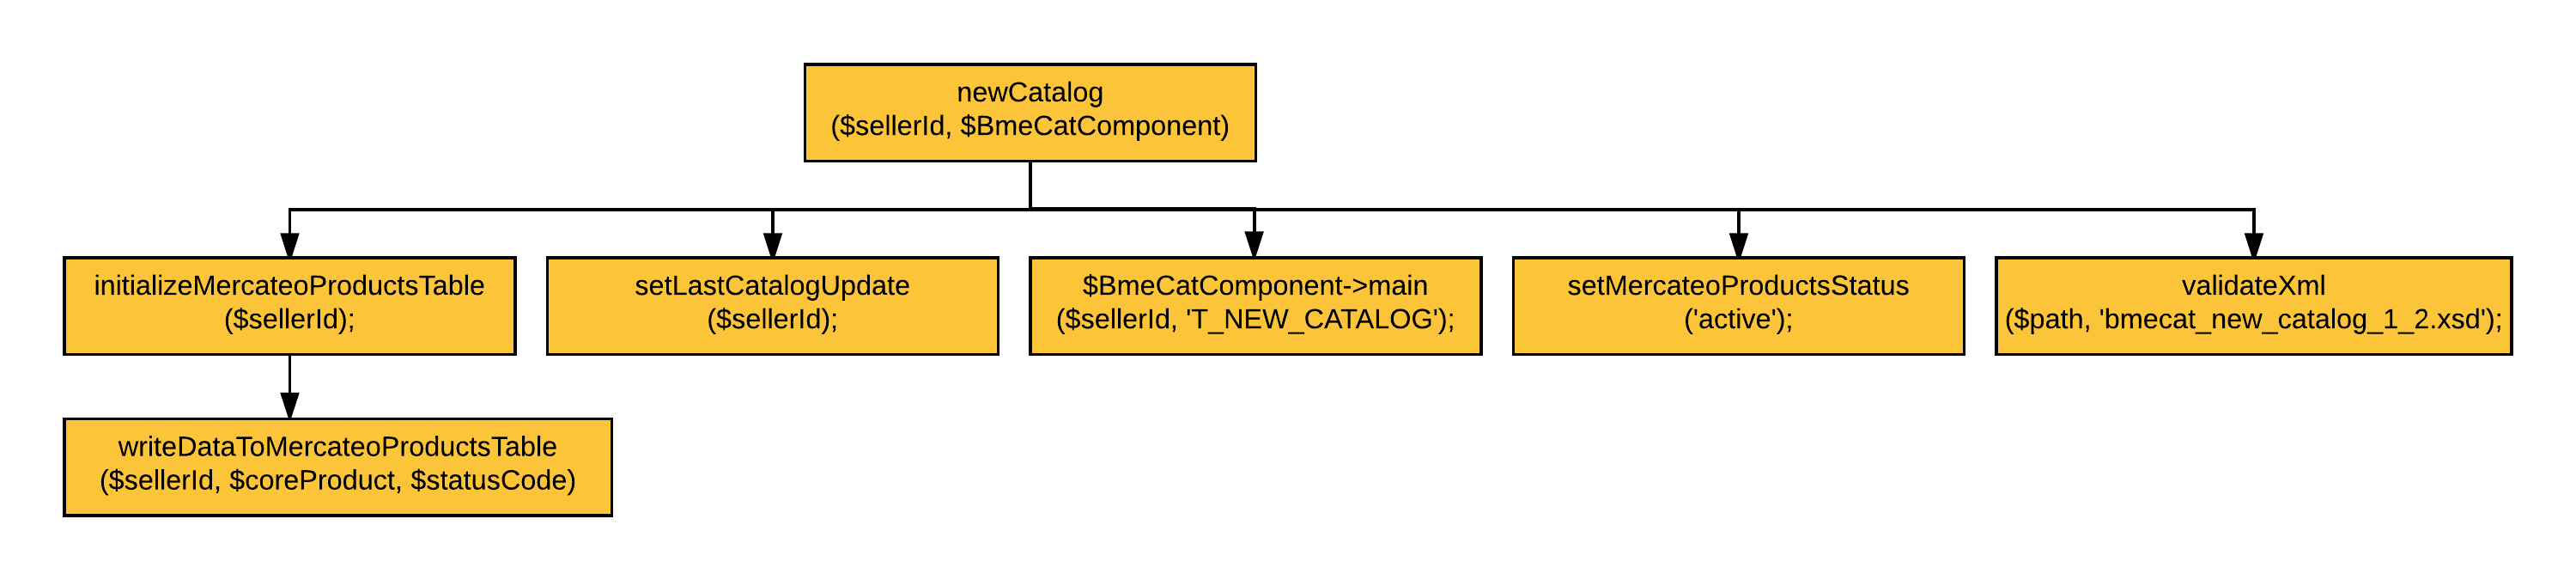
\includegraphics[width=1 \linewidth]{img/newCatalogAufrufhierarchie}
		\captionof{figure}[BasicLogic]{Aufrufhierarchie der Methode \texttt{newCatalog}}
		\vspace{1em}
	\end{minipage}

	
	Mit \texttt{initializeMercateoProductsTable(\$sellerId)} wird die \texttt{mercateo\_products} Tabelle initialisiert. Dabei werden die in \texttt{core\_products} gespeicherten Produkte des angegebenen Verkäufers geladen und durch Aufruf von \texttt{writeDataToMercateoProductsTable} in die \texttt{mercateo\_products} Tabelle geschrieben. Der Variablen \texttt{statusCode} wird dabei der Wert \textit{new} zugewiesen. 
	
	Anschließend wird mit \texttt{setLastCatalogUpdate} der Timestamp der Katalogerzeugung in die \texttt{core\_configurations} Tabelle geschrieben.
		
	Durch Aufruf der Methode \texttt{createBMECatXMLDocument(\$sellerId, \$transactionType, \$prevVersion = null)} des \texttt{BmeCatComponent}-Objektes wird die zu erzeugende XML-Datei geschrieben . Dem Parameter \texttt{transactionType} wird hier der Wert \texttt{T\_NEW\_CATALOG} zugewiesen. Anschließend wird mit \texttt{setMercateoProductsStatus(\$status)} der \textit{status} aller in \texttt{mercateo\_products} gespeicherten Artikel auf \textit{active} gesetzt.

	Die Validierung des soeben erzeugten Dokumentes erfolgt mit dem Schema \texttt{bmecat\_new\_catalog\_1\_2.xsd} durch Aufruf von \texttt{validateXml(\$path, \$schemePath)}.
	
	
	
	\subsubsection{Erzeugung eines Update-Katalogdokumentes  mit der Klasse \texttt{UpdateCatalogTask}}
	
	Die Klasse \texttt{UpdateCatalogTask} dient der Erzeugung eines Update-Katalog-Dokumentes. Die \texttt{initialize()} Methode verhält sich wie im vorherigen Abschnitt beschrieben. Auch die \texttt{main()} verhält sich ähnlich, mit dem Unterschied, dass nun positiv darauf geprüft wird, ob die \texttt{mercateo\_products} Tabelle bereits Einträge des angegebenen Verkäufers enthält. \\
	\begin{minipage}{\linewidth}
		\vspace{1em}
		\centering
		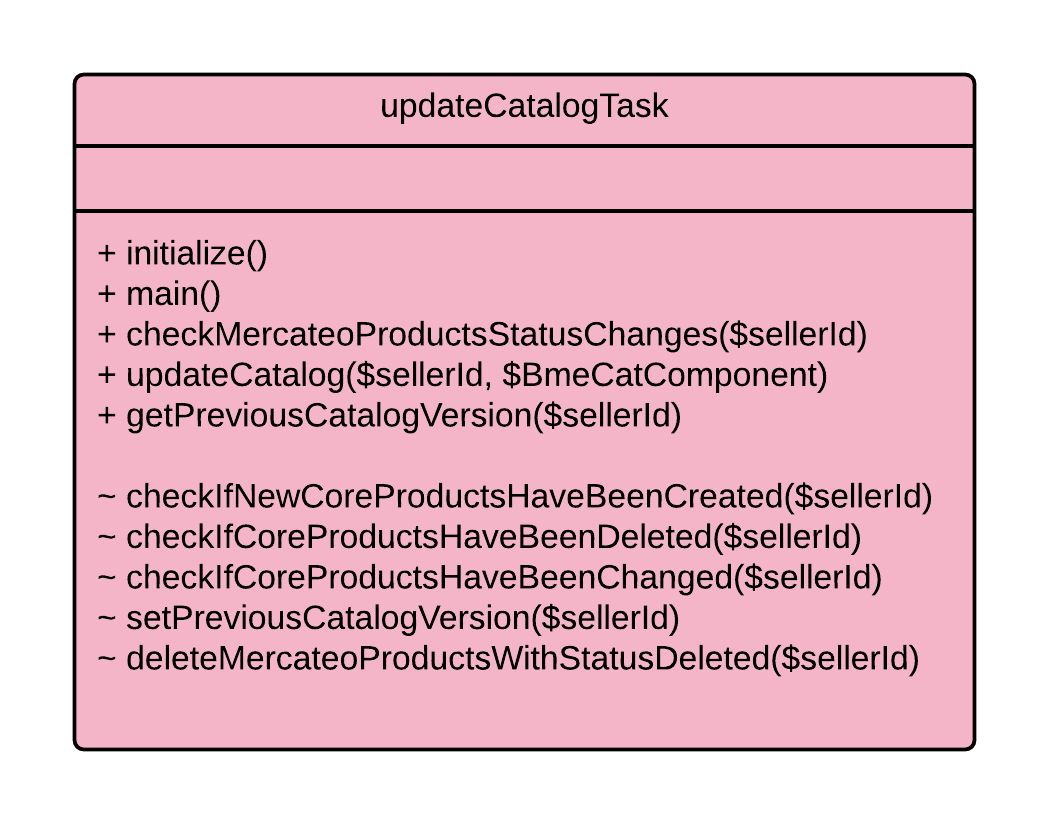
\includegraphics[width=0.7 \linewidth]{img/UpdateCatalogTaskUML}
		\captionof{figure}[BasicLogic]{UML-Klassendiagramm der Klasse \texttt{UpdateCatalogTask}}
		\vspace{1em}
	\end{minipage}
	
	Die Funktion \texttt{checkMercateoProductsStatusChanges(\$sellerId)} fasst
 	jene 3 Methoden zusammen, die prüfen ob Produkte gelöscht, geändert oder neu hinzugefügt wurden. Diese geben jeweils \texttt{true} zurück, falls eine entsprechende Änderung stattgefunden hat. Zugleich wird in der Konsole eine Meldung der Form 	
		\begin{lstlisting}
		Info: Product with CoreProductId: 1781 added
		Info: Product with CoreProductId: 1782 deleted
		Info: Product with CoreProductId: 1783 updated
		\end{lstlisting} ausgegeben, die zudem in der Datei \textit{productChange.log} erfasst wird.
			
		Die Methode \texttt{checkIfNewCoreProductsHaveBeenCreated(\$sellerId)} überprüft ob es seit der letzten Katalogerstellung in der Tabelle \texttt{core\_products} neue Einträge gab. Dazu wird die Tabelle \texttt{mercateo\_products} über einen LEFT-JOIN an \texttt{core\_products} gebunden. All jene Produkte aus \texttt{core\_products}, deren \textit{core\_product\_id} nicht in \texttt{mercateo\_products} zu finden ist müssen als neu gelten und werden demnach mit dem Statuscode \texttt{new} in \texttt{mercateo\_products} geschrieben. 
		
	
		Mit \texttt{checkIfCoreProductsHaveBeenDeleted(\$sellerId)} wird geprüft ob Daten aus der \texttt{core\_products} Tabelle gelöscht wurden. Auch hier wird \texttt{mercateo\_products} über einen LEFT-JOIN an \texttt{core\_products} gebunde. All jene Produkte deren \textit{core\_product\_id} 
		noch in der \texttt{mercateo\_products} Tabelle vermerkt ist, nicht aber in \texttt{core\_products}, müssen als gelöscht gelten. Entsprechend wird der Status der betroffenen Produkte in \texttt{mercateo\_products} auf \texttt{delete} gesetzt.
		
		Durch die Methode \texttt{checkIfCoreProductsHaveBeenChanged(\$sellerId)} schließlich wird geprüft ob sich Produktdaten seit der letzten Katalogerstellung geändert haben. Dazu wird die Tabelle \texttt{core\_product\_updates} über einen INNER-JOIN an \texttt{mercateo\_products} gebunden.
		Beim Erstellen des Kataloges wurde der Zeitpunkt der Erzeugung in der \texttt{core\_configurations} Tabelle gespeichert. All jene Einträge aus \texttt{core\_product\_updates}, deren Erzeugungsdatum nach der letzten Katalogerstellung liegt werden in \texttt{mercateo\_products} mit dem Status \texttt{update} versehen.
	
	Hat eine der soeben vorgestellten Methoden \texttt{true} zurückgeliefert, wird die Methode \texttt{UpdateCatalog(\$sellerId, \$BmeCatComponent)} aufgerufen, die alle an der Erstellung eines Update-Katalogdokumentes beteiligten Methoden zusammenfasst.
	
	\begin{minipage}{\linewidth}
		\vspace{1em}
		\centering
		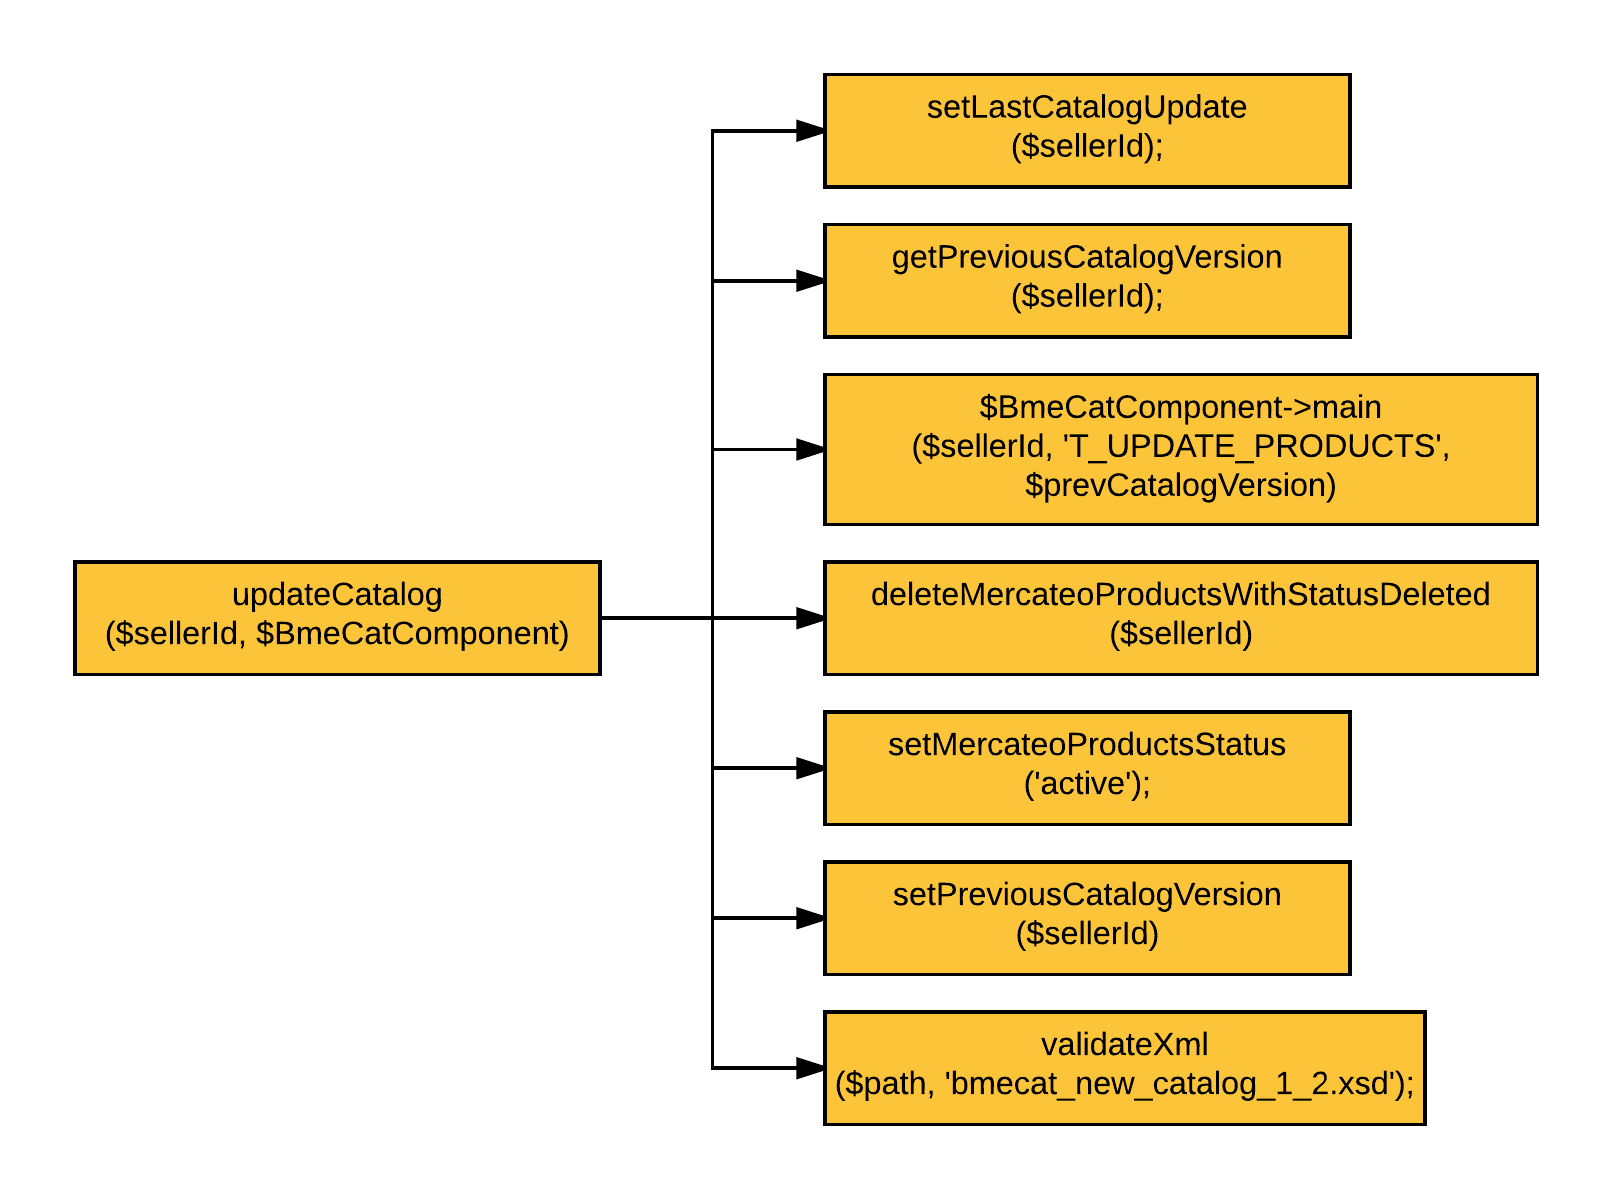
\includegraphics[width=0.7 \linewidth]{img/updateKatalogAufrufhierarchie}
		\captionof{figure}[BasicLogic]{Aufrufhierarchie der Methode \texttt{UpdateCatalog}}
		\vspace{1em}
	\end{minipage}
	
	Zu Beginn wird mit \texttt{setLastCatalogUpdate(\$sellerId)} der Zeitpunkt der Katalogerstellung in der \texttt{core\_configurations} Tabelle gespeichert.  
	
	Die Methode \texttt{getPreviousCatalogVersion(\$sellerId)} liefert den in \texttt{core\_configurations} gespeicherten Wert des bei der Transaktion \texttt{T\_UPDATE\_PRODUCTS} benötigten Attributes \texttt{prev\_version} zurück. Existiert noch kein Eintrag in der Tabelle wird dieser erstellt und der Wert des Attributes auf \enquote{0} gesetzt. Bei der ersten Ausführung von \texttt{T\_UPDATE\_PRODUCTS} wird so stets \enquote{0} zurückgeliefert. Dieser Wert wird in der Variablen \texttt{\$prevCatalogVersion} gespeichert um bei Aufruf der BMECatComponent-Methode \texttt{createBMECatXMLDocument} - diesmal wird der Parameter \texttt{\$transactionType} mit \texttt{T\_UPDATE\_PRODUCTS} initialisiert - übergeben werden zu können.
	
	Wurde der Updatekatalog erstellt müssen die Einträge aus der \texttt{mercateo\_products} Tabelle gelöscht werden, deren Status auf \texttt{delete} gesetzt ist. Die Methode \texttt{deleteMercateoProductsWithStatusDeleted(\$sellerId)} setzt dies um.
	
	Anschließend bekommen die verbliebenen Einträge den Status \texttt{active} zugewiesen.Mit \texttt{setPreviousCatalogVersion(\$sellerId)} wird der entsprechende Wert in \texttt{core\_configurations} um 1 erhöht.
	
	Die Validierung des Katalogdokumentes erfolgt diesmal mit dem Schema \texttt{bmecat\_update\_products\_1\_2.xsd}.
	
	\subsubsection{Die Klasse DeleteCatalogTask}
	
	Das Löschen von Produkten eines bestimmten Verkäufers wird mit der Klasse \texttt{DeleteCatalogTask} realisiert. 
	
	\begin{minipage}{\linewidth}
		\vspace{1em}
		\centering
		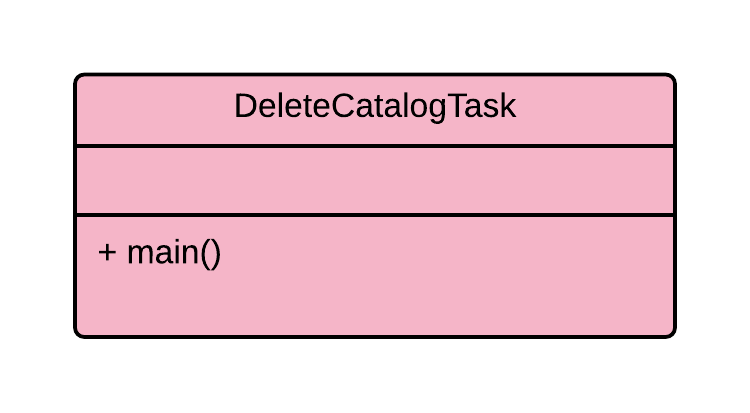
\includegraphics[width=0.4 \linewidth]{img/DeleteCatalogTask}
		\captionof{figure}[BasicLogic]{Klassendiagramm DeleteCatalogTask}
		\vspace{1em}
	\end{minipage}	
	
	In der \texttt{main()}-Methode wird die Validierung des übergebenen Arguments durchgeführt und der Nutzer gefragt, ob er sich seines Handelns sicher ist. Falls ja, werden mit deleteSellersArticlesFromMercateoProductsTable(\$sellerId) die Produkte des entsprechenden Verkäufers aus der \texttt{mercateo\_products}-Tabelle gelöscht.

	\subsubsection{Ressourcenmanagement}
	
	Die XML-Knoten im BMECat-Dokument können auch, teilweise komfortabler, mit anderen in PHP zur Verfügung stehenden XML-Manipulationsklassen (wie z.B.  DOMDocument) geschrieben werden. Bei der Verwendung der DOMDocument Klasse wird zunächst der komplette Objektbaum aufgebaut und im Arbeitsspeicher gehalten, bevor das XML-Dokument geschrieben werden kann. Bei mehreren zehntausend zu exportierenden Produkten kann es so passieren, dass der zur Verfügung stehende Arbeitsspeicher nicht mehr ausreicht bzw. verhältnismäßig viel Speicher beansprucht wird. Die Verwendung der XMLWriter-Klasse gestattet es die Anzahl der im Schreibpuffer gehaltenen Elemente zu limitieren und diese bei Erreichen der Obergrenze zu schreiben um anschließend den Puffer zu leeren. Dadurch wird der Speicherverbrauch beim Schreibvorgang drastisch reduziert. 
		
	Lese- und Schreibzugriffe auf die Datenbank erfolgen stets sequentiell, wie folgendes Codebeispiel illustriert:
	\lstset{language=php}
	\begin{lstlisting}[]
	$limit = 100;
	$page = 1;
	
	do {
	    $products = $this->CoreProducts->find('all')
	        ->where($conditions)
	        ->limit($limit)
	        ->page($page);
	        
	    if (!empty($products)) {
	        foreach ($products as $product) {        
	            $this->writeDataToMercateoProductsTable($product->id, 'new');
	        }
	    }$page++;
	} while (count($products->toArray()) == $limit);
	\end{lstlisting} 
	Durch diese Maßnahme wird der Speicherverbrauch bei Datenbankzugriffen klein gehalten.
	
	\subsection{Bestandsdatenabfrage}
	
	Die Bestandsdatenabfrage ist in der Controllerklasse \texttt{AvailabilityController} implementiert.
	
	\begin{minipage}{\linewidth}
		\vspace{1em}
		\centering
		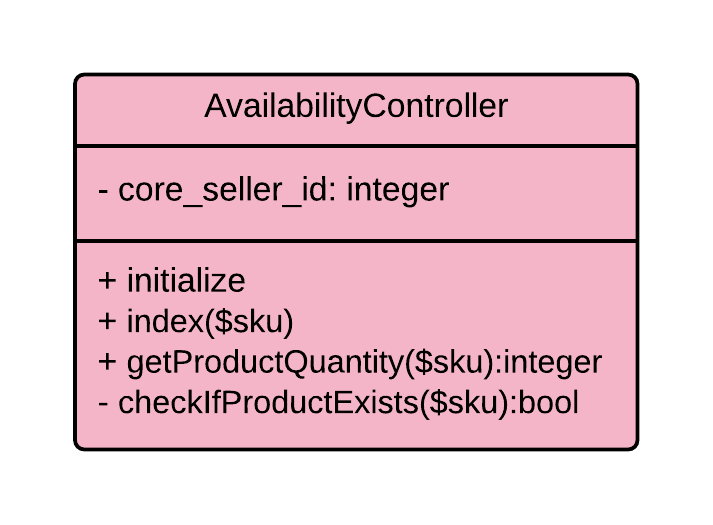
\includegraphics[width=0.4 \linewidth]{img/AvailabilityControllerUML}
		\captionof{figure}[BasicLogic]{Klassendiagramm AvailabilityController}
		\vspace{1em}
	\end{minipage}
	
	Für das Zurückliefern der Bestandsdaten einer angefragten SKU wird keine View benötigt. CakePHP versucht jedoch automatisch zu jeder aufgerufenen Controllermethode eine entsprechende View zu rendern \footnote{vgl. hierzu Kapitel 1.3.1 - Convention over Configuration in CakePHP}.  Da jedoch dennoch auf die \texttt{index(\$sku)} Methode zugegriffen werden soll wird in der Funktion \texttt{initialize} das automatische Rendern einer View abgeschaltet, sowie der direkte Zugriff auf die texttt{index(\$sku)} Methode gestattet.
	
	Die Funktion \texttt{checkIfProductExists(\$sku)} prüft zunächst ob sich das angefragte Produkt in der \texttt{mercateo\_products} Tabelle finden lässt.Ist dies der Fall, wird zusätzlich geprüft ob es auch in der \texttt{core\_products} Tabelle gefunden werden kann. Falls beides zutrifft, wird \texttt{true} zurückgeliefert, andernfalls \texttt{false}.
	
	Die \texttt{index(\$sku)} Methode verarbeitet die Anfrage. Kann das angefragte Produkt in der Datenbank gefunden werden,wird über Aufruf der Methode \texttt{getProductQuantity(\$sku)}) die Bestandsmenge desselben abgefragt und als Text im Browserfenster ausgegeben. Zusätzlich wird der HTTP-Statuscode \textit{200} zurückgeben um das anfragenden System darüber zu informieren, dass die Anfrage erfolgreich bearbeitet werden konnte.
	
	Können keine Produkdaten gefunden werden, wird im Browserfenster eine entsprechende Browsermeldung ausgegeben und der HTTP-Statuscode \textit{204} zurückgeben. Das anfragende System erlangt so Kenntnis darüber, dass die Anfrage verabeitet werden konnte, jedoch kein Inhalt zurückgeliefert werden kann.
	
	\section{Test}
	
	
	CakePHP unterstützt \enquote{ab Werk} Unit Testing mit PHPUnit, welches in vorliegender Arbeit verwendet wird. -ETWAS ÜEBR DIE KONVENTIONEN SCHREIBEN-  Um jene Methoden testen zu können die lesend und schreibend auf die Datenbank zugreifen, werden für die betroffenen Tabellen \textit{Fixtures} erstellt. Fixtures sind Duplikate der eigentlichen Tabellen und enthalten Testdatensätze. Der Vorteil von Fixtures ist, dass Datenbankabfragen durchgeführt werden können ohne, dass die eigentlichen Datensätze davon betroffen wären.
	
	Im folgenden werden die einzelnen Testklassen und Testfälle vorgestellt.
	
	\subsection{Die Klasse AvailabilityControllerTest}
	
	Um die Methoden \texttt{getProductQuantity} und \texttt{checkIfProductExists} testen zu können müssen Fixtures für die Tabellen \texttt{mercateo\_products}, \texttt{core\_products}, \texttt{core\_marketplaces} und \texttt{core\_product\_quantities} erstellt und mit Testdatensätzen befüllt werden.
	\texttt{testCheckIfProductExists()} enthält je einen Positiv- und einen Negativtest. Es wird erwartet, dass die Methode \texttt{checkIfProductExists} den booleschen Wert \texttt{true} zurückliefert, falls ein Produkt in der Datenbank gefunden werden konnte und \texttt{false}, wenn nicht.
	Die Methode \texttt{testGetProductQuantity} prüft ob der Rückgabewert dem erwarteten Zahlenwert entspricht und ob er vom Typ \textit{Integer} ist.
	
	\subsection{Die Klasse UpdateCatalogTaskTest}
	
	In der Klasse \texttt{UpdateCatalogTaskTest} werden folgende Fixtures geladen:
	\begin{itemize}[nosep]
		\item \texttt{core\_configurations}
		\item \texttt{mercateo\_products}
		\item \texttt{core\_products}
		\item \texttt{core\_product\_quantities}
		\item \texttt{core\_product\_types}
		\item \texttt{core\_product\_updates}
	\end{itemize}
	\texttt{testGetPreviousCatalogVersion()} testet positiv und negativ auf einen in der \texttt{core\_configuartions}-Fixture hinterlegten Konfigurationswert. Zudem wird geprüft, ob \enquote{0} zurückgeliefert wird, falls für den angegeben Seller noch kein Konfigurationswert in der Datenbank angelegt wurde.
	
	Mit \texttt{testCheckMercateoProductsStatusChanges()} werden die als \textit{private} ausgezeichneten Methoden \texttt{checkIfNewCoreProductsHaveBeenCreated}, 
	\texttt{checkIfCoreProductsHaveBeenDeleted} und
	\texttt{checkIfCoreProductsHaveBeenUpdated} auf Funktion getestet. Für Testfall 1 - jeweils ein Produkt wurde hinzugefügt, gelöscht bzw. aktualisiert- werden entsprechende Einträge in den Fixturetabellen von \texttt{core\_products}, \texttt{mercateo\_products} und \texttt{core\_product\_updates} angelegt. Als Rückgabewert wird demzufolge \texttt{true} erwartet. Entsprechendes geschieht für den Fall, dass keine Produktstatusveränderungen stattgefunden haben sollen und als Rückgabewert \texttt{false} erwartet werden kann.
	
	\subsection{Die Klasse MercateoAccountsTableTest}
	
	Die Funktion \texttt{validateCatalogVersionFormat(\$value)} erweitert die CakePHP Standardvalidatormethoden. Mittels regulärem Ausdruck wird geprüft ob die übergeben Zeichenkette einem bestimmten Format entspricht. \texttt{testValidateCatalogVersionFormat()} führt einen Positiv- und einen Negativtest der Funktionalität durch. 
	
	\subsection{Die Klasse BMECatComponentTest}
	
	Um die Methoden \texttt{getSellerName(\$sellerId)} und \texttt{getParentCoreCategoryIds(\$sellerId)} testen zu können werden die Fixtures für \texttt{core\_sellers} und \texttt{core\_categories} geladen.
	\texttt{testGetSellerName()} prüft mit einem Positiv- und einem Negativtest ob die zurückgelieferte Zeichenkette der Erwartung entspricht.
	
	Die Methode \texttt{testGetParentCoreCategoryIds()} prüft ob ein Array zurückgeliefert wird und ob die darin gespeicherten Werte vom Typ \textit{Integer} sind.
	
	\texttt{testArticleDataValidator()} führt einen Positiv- und einen Negativtest durch, indem jeweils eine \enquote{gültige} bzw. \enquote{ungültige} Instanz von \textit{CoreProducts} an \texttt{articleDataValidator(\$product)} übergeben wird.
	
	Mit \texttt{testCheckImageFormat()} wird geprüft, ob \texttt{checkImageFormat(\$image)} jeweils \texttt{true} zurückliefert, wenn der übergebene \textit{URI} auf \enquote{.jpeg}, \enquote{.jpg} oder \enquote{gif} endet. Es wird \texttt{false} erwartet, wenn die Datei eine andere Endung hat.
	
	
	
	

	

